\documentclass[a4paper, 12pt]{article}
\usepackage[utf8]{inputenc}
\usepackage[spanish]{babel} 
\usepackage{amsmath}
\usepackage{graphicx}
\usepackage{fancyhdr}
\usepackage{imakeidx}
\usepackage{dirtree}
\usepackage{float}
\usepackage{caption}
\captionsetup[figure]{labelformat=empty}

\usepackage[linesnumbered]{algorithm2e}
\SetKwRepeat{Do}{do}{while}%

\usepackage{xcolor}
\usepackage{listings}
\lstset{basicstyle=\ttfamily,
  showstringspaces=false,
  commentstyle=\color{red},
  keywordstyle=\color{blue}
}


\title{
\textbf{Metaheurística - Práctica 3.a} \\
Búsquedas por Trayectorias para el Problema de la Asignación Cuadrática
}

\author{
3º Grado Ingeniería Informática, Grupo 3 (Miércoles)\\
Salvador Corts Sánchez, 75935233C \\
salvacorts@correo.ugr.es
}

\date{}

\fancyhead[LE,RO]{Salvador Corts Sánchez, 75935233C}
\fancyhead[RE,LO]{QAP: Práctica 3}
\pagestyle{fancy}

\setcounter{tocdepth}{4}
\setcounter{secnumdepth}{4}
\makeindex

\begin{document}
   % Header
   \maketitle
   
   % Index
   \newpage
   \tableofcontents

   
   % Descripción del problema
   \newpage
   \section{Descripción del problema}
   El problema de asignación cuadrática (en inglés, quadratic assignment problem, QAP) es uno de los problemas de optimización combinatoria más conocidos. En él se dispone de n unidades y n localizaciones en las que situarlas, por lo que el problema consiste en encontrar la asignación óptima de cada unidad a una localización. La nomenclatura “cuadrático” proviene de la función objetivo que mide la bondad de una asignación, la cual considera el producto de dos términos, la distancia entre cada par de localizaciones y el flujo que circula entre cada par de unidades. El QAP se puede formular como:
   
   $$QAP = 
\begin{matrix}
min\\
\pi \in \prod_N 
\end{matrix}   \Bigg( \sum_{i=1}^{n} \sum_{j=1}^{n} f_{ij}d_{\pi(i)\pi(j)} \Bigg)   
   $$
   
   donde:
   \begin{itemize}
      \item \textbf{$\pi$} es una solución al problema que consiste en una permutación que representa la asignación de la unidad $i$ a la localización  $\pi(i)$.
      
      \item $f_{ij}$ es el flujo que circula entre la unidad $i$ y la $j$.
      
      \item $d_{kl}$ es la distancia existente entre la localización $k$ y la $l$.
   \end{itemize}
   
   
   % Descripción de la aplicación de los algoritmos
   \newpage
   \section{Consideraciones comunes a los algoritmos utilizados}
   Esta práctica ha sido diseñada como una librería de metaheurísticas per se. Es decir, existe un tipo de objeto \textbf{Solution} y un tipo de objeto \textbf{Solver} del cual heredarán los objetos que implementan las diversas metaheurísticas. Cada metaheurística deberá implementar la función \textit{Solve} que devuelve un objeto \textbf{Solution}.
   
   \vspace*{0cm}
   \begin{figure}[H]
      \centering
      \hspace*{-3.5cm}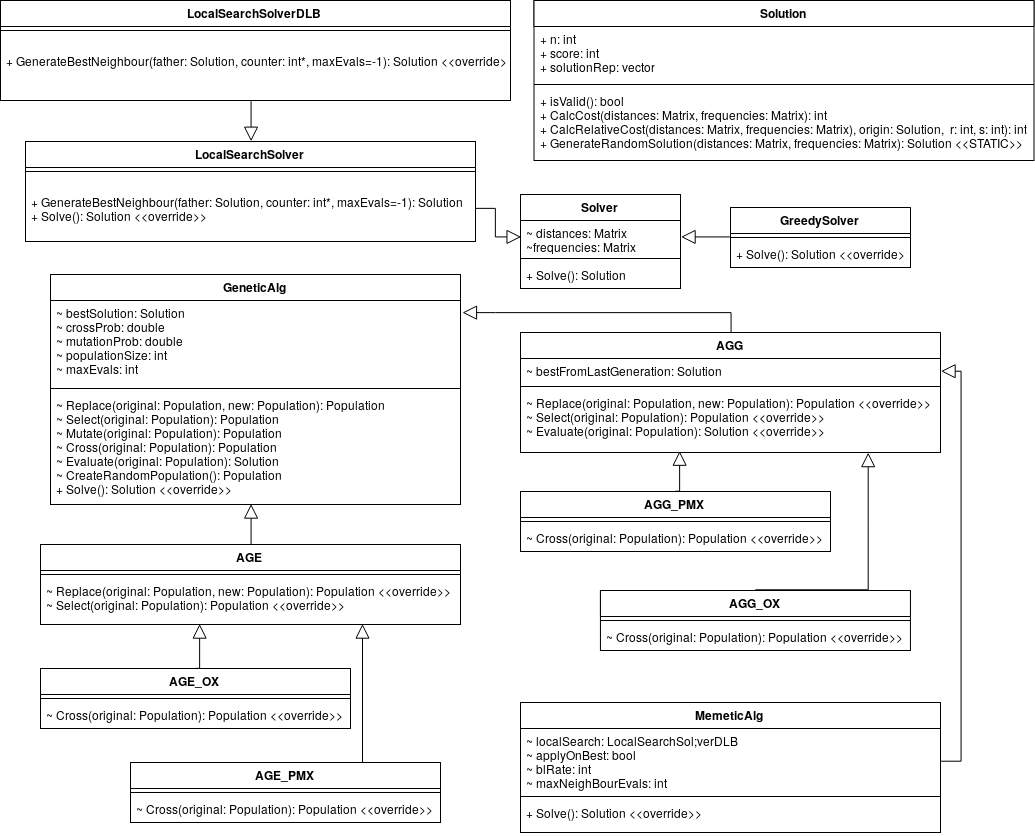
\includegraphics[scale=0.4]{mhClassDiagram}
      \caption{Diagrama de clases}
   \end{figure}
   
   \newpage
   \subsection{Clase Solver}
   Esta clase debe ser heredada por las metaheurísticas a implementar. Su representación consta de dos matrices:
   \begin{itemize}
      \item \textbf{Distancias}: Matriz de distancias entre un punto $i$ y otro $j$.
      \item \textbf{Frecuencias}: Matriz de flujo entre un objeto $i$ y otro $j$. 
   \end{itemize}
   Tiene una función virtual llamada \textit{Solve} que ha de ser implementada por los objetos que hereden de \textbf{Solver}. Es la interfaz común a todos los objetos de tipo Solver para obtener una Solución.

   \subsection{Clase Solution}
   Sirve para representar una solución, la cual, se implementa como un vector donde cada posición $i$ representa un objeto y alberga la localización $j$ donde debe ser colocado dicho objeto $i$. 
   
   \begin{center}
      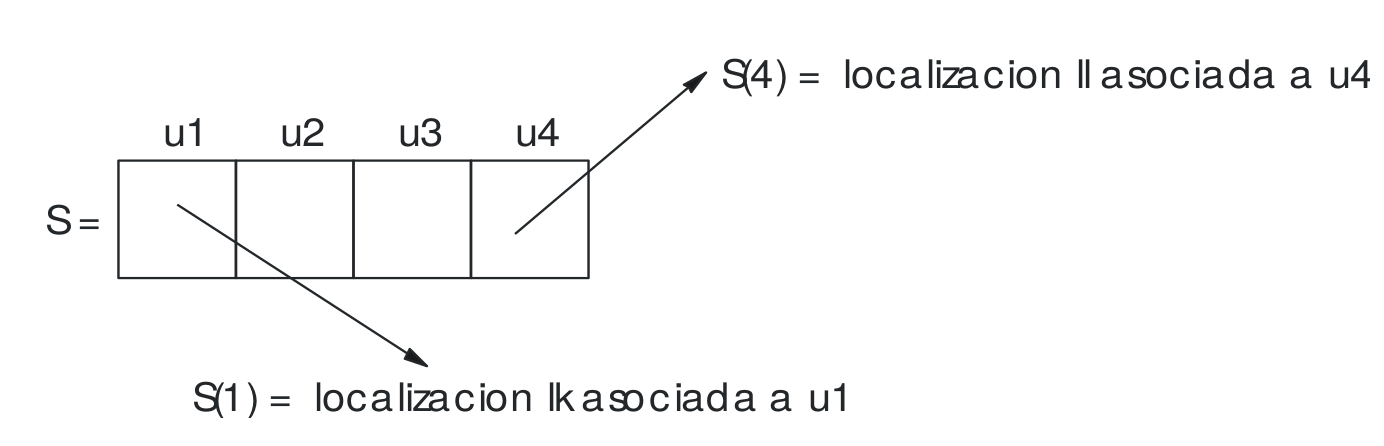
\includegraphics[scale=0.14]{solRep}
   \end{center}
   
   Existe una función \textit{CalcCost} que calcula el coste de dicha solución como:
      $$cost = \sum_{i=1}^{n}\sum_{j=1, j \neq i}^{n} f_{ij}d_{\pi(i)\pi(j)}$$
   donde:
   \begin{itemize}
      \item $\pi$ es la solución al problema.
      
      \item $f_{ij}$ es el flujo que circula entre la unidad $i$ y la $j$.
      
      \item $d_{kl}$ es la distancia existente entre la localización $k$ y la $l$.
   \end{itemize}\vspace*{0.5cm}
   
   Dado que el cálculo del coste de la solución es bastante costoso, $O(n^{2})$, Esta función debe llamarse manualmente al menos una vez para obtener el coste y que este se guarde en la representación de la clase.
   
   
   \newpage
   \section{Algoritmo Greedy}
   Se basa en el cálculo de los potenciales de flujo y distancia definidos como:
   \begin{center}
      $\hat{f}_i = \sum_{j=1}^{n}f_{ij}$ \hspace*{1cm} $\hat{d}_i = \sum_{j=1}^{n}d_{ij}$
   \end{center}
   
   El algoritmo irá seleccionando la unidad $i$ libre con mayor $\hat{f}_i$ y le asignará la localización $j$ libre con menor $\hat{d}_j$. Su implementación en pseudocódigo es la siguiente:  
      \begin{algorithm}
      	\caption{greedy.cpp - GreedySolver::Solve}
      	
          \# Calcula los potenciales\\
          $dp = fp = vector(n)$\\
          \For{$i=1$ \KwTo $n$}{
             $\hat{f}_i = \hat{d}_i = 0$\\
             \For{$j=0$ \KwTo $n$}{
                $\hat{f}_i = \hat{f}_i + f_{ij}$\\
                $\hat{d}_i = \hat{d}_i + d_{ij}$\\
             }
             $dp_i = \hat{d}_i$\\
             $fp_i = \hat{f}_i$\\
          }\vspace*{0.1cm}
          
          \# Calcula la mejor combinación. $\pi$ es la representación de la solución\\
          $locAssigned = unitAssigned = vector(n)\{0\}$\\
          \For{$i=1$ \KwTo $n$}{
             $best\hat{f} = -\infty$;\hspace*{0.5cm}$best\hat{f}_{index}=0$\\
             $best\hat{d} = \infty$;\hspace*{0.5cm}$best\hat{d}_{index}=0$\\
             \For{$j=0$ \KwTo $n$}{
                $\hat{f}_i = fp_j$;\hspace*{0.5cm}$\hat{d}_i = dp_j$\\
                
                \If{$\hat{f}_i > best\hat{f}$ \textbf{and} $unitAssigned_j \neq 1$}{
                   $best\hat{f} = \hat{f}_i$;\hspace*{0.5cm}$best\hat{f}_{index}=j$\\
                }
                
                \If{$\hat{d}_i < best\hat{d}$  \textbf{and} $locAssigned_j \neq 1$}{
                   $best\hat{d} = \hat{d}_i$;\hspace*{0.5cm}$best\hat{d}_{index}=j$\\
                }
             }
             $\pi(best\hat{f}_{index}) = best\hat{d}_{index}$\\
             $unitAssigned_{best\hat{f}_{index}} = locAssigned_{best\hat{d}_{index}} = 1$\\             
          }
      \end{algorithm}
      
      
      \newpage
      \section{Algoritmo de Búsqueda Local}
      Vamos a utilizar una \textbf{búsqueda local del primer mejor}. Cuando se genera una solución vecina que mejora a la actual, se toma esta como solución y se pasa a la siguiente iteración. Se detiene la búsqueda cuando no se genera ningún vecino mejor que la solución actual. La implementación de dicha idea, que será la función \textit{Solve}, se puede ver como:
      \begin{algorithm}
		\caption{localSearch.cpp - LocalSearchSolver::Solve}      
      
         $\pi = GenerateInitialSolution()$ \# Será aleatoria\\
         \Do{$\exists \pi'$}{
            $\pi' = GenerateBestNeighbour(\pi)$
            
            \lIf{$\exists \pi'$}{$\pi = \pi'$}
         }
      \end{algorithm}
      
      A fin de minimizar el riesgo de quedarnos en un óptimo local, vamos a partir de una solución aleatoria en vez de partir de una solución greedy. Dicha solución aleatoria se genera de la siguiente manera:
      \begin{algorithm}
      	\caption{solution.cpp - Solution::GenerateRandomsolution}
         $assigned = vector(n)\{0\}$\\
         \For{$i=1$ \KwTo $n$}{
            \Do{$assigned_r \neq 0$}{
               $r = random() \ mod\ n$\\
             }
             
             $\pi(i) = r$\\
             $assigned_r = 1$\\
         }
      \end{algorithm}
      
      Como se comentó anteriormente, el proceso de cálculo del coste de la solución es de orden cuadrático por lo que realizar dicho calculo con cada vecino es sumamente costoso; En su lugar, vamos a considerar una \textbf{factorización} (con eficiencia $O(n)$) teniendo en cuenta solo los cambios realizados por el movimiento de intercambio para generar el vecino. El incremento del coste de cambiar el elemento en la posición r $r$ por el de $s$ se define como:
      $$
\Delta C(\pi,r,s) = \sum_{k=1, k\neq r,s}^{n}\begin{bmatrix}
f_{rk}(d_{\pi(s)\pi(k)} - d_{\pi(r)\pi(k)}) + f_{sk}(d_{\pi(r)\pi(k)} - d_{\pi(s)\pi(k)}) +\\ 
f_{kr}(d_{\pi(k)\pi(s)} - d_{\pi(k)\pi(r)}) + f_{ks}(d_{\pi(k)\pi(r)} - d_{\pi(k)\pi(s)})
\end{bmatrix} 
      $$
      
      \newpage
      Si $\Delta C(\pi,r,s) < 0$, el resultado de cambiar $r$ por $s$ es favorable, es decir, el costo es menor por lo que tomaremos el vecino resultante de este cambio como solución actual y generamos nuevos vecinos a partir de este.\\
      
      La función que hace uso de esta factorización para explorar los vecinos de una solución se implementaría como:
      \begin{algorithm}
      	\caption*{localSearch.cpp-LocalSearchSolver::GenerateBestNeighbour}
         \SetKwProg{Def}{def}{:}{end}
         \Def{GenerateBestNeighbour($\pi$)}{
            \For{$r=1$ \KwTo $n/2$}{
               \For{$s=r+1$ \KwTo $n$}{                  
                  \If{$\Delta C(\pi,r,s) < 0$}{
                     $\pi' = \pi$\\
                     $t = \pi'(r)$\\
                     $\pi'(r) = \pi'(s)$\\
                     $\pi'(s) = t$\\
                     
                     \textbf{return} $\pi'$
                  }
               }
            }         
         }
      \end{algorithm}
      
      Como vemos, podemos reducir considerablemente el numero de iteraciones totales iterando en $r$ en el primer bucle hasta $n/2$ y en el segundo desde $r+1$ hasta $n$, ya que así podemos evitar comparar dos veces el mismo movimiento. Es lo mismo cambiar $r$ por $s$ que $s$ por $r$.
     
      
      \newpage
      \subsection{Búsqueda Local con \textit{Don't Look Bits}}
      Como estamos utilizando una \textbf{búsqueda local del primer mejor}, podemos definir una lista de candidatos a la que llamamos \textbf{\textit{Don't Look Bits}} que reducirá significativamente el tiempo de ejecución.\\
      
      Se trata de un un vector de bits inicialmente a 0, esto nos indica que todos los movimientos pueden ser considerados. Si tras probar todos los movimientos asociados un bit no hemos encontrado ninguna mejora, cambiaremos el valor de dicho bit a 1, indicando que esta unidad no debe ser tenida en cuenta hasta que dicha unidad asociada a ese bit se vea implicada en un movimiento que mejora la solución actual, en cuyo caso el bit será nuevamente 0.\\
      
      Podemos ejemplificar este algoritmo con el siguiente pseudocódigo:
      \begin{algorithm}
         $dlbMask = vector(n)\{0\}$ \# Don't look bits\\
         \SetKwProg{Def}{def}{:}{end}
         \Def{GenerateBestNeighbour($\pi$)}{
            \For{$r=1$ \KwTo $n$}{
               \lIf{$dlbMask_r \neq 0$}{\textbf{continue}}
               \For{$s=1$ \KwTo $n$}{                  
                  \If{$\Delta C(\pi,r,s) < 0$}{
                     $\pi' = \pi$\\
                     $t = \pi'(r)$\\
                     $\pi'(r) = \pi'(s)$\\
                     $\pi'(s) = t$\\
                     
                     $dlbMask_r = dlbMask_s = 0$\\
                     \textbf{return} $\pi'$
                  }
               }
               $dlbMask_r = 1$
            }         
         }
      \end{algorithm}
      
      
      \newpage
      \section{Algorítmos Genéticos}      
      Se han implementado dos tipos de algorítmos genéticos:
      \begin{itemize}
      	\item Generacionales.
      	\item Estacionarios.
      \end{itemize}
       
       Ambos comparten los operadores de \textbf{Mutación}, \textbf{Cruce} y \textbf{Evaluación} así como la del \textbf{método de búsqueda}. La diferencia entre ambos está en los operadores de \textbf{Selección} y \textbf{Remplazo} que se explicarán a fondo mas tarde.\\
       
       Estos operadores actuan sobre una Población compuesta de $n$ cromosomas. Es decir, un conjunto (vector) de $n$ soluciones diferentes que modificaremos, mezclaremos y compararemos a fin de encontrar la solución más óptima posible sorteando óptimos locales. 
       
       \subsubsection*{Método de búsqueda de un algorítmo genético}
       Partiremos de una población generada aleatoriamente creando, con la función descrita en el apartado 4. (Búsqueda Local), tantos cromosomas soluciones como tamaño de la población deseemos.
       \begin{algorithm}
       	\caption{\textit{genetic.cpp} - GeneticAlg::CreateRandomPopulation}
       	
         \SetKwProg{Def}{def}{:}{end}
         \Def{GenerateRandomPopulation()}{
         	$P = Population(n)\{0\}$ \# Población de $n$ cromosolmas\\
            \For{$i=1$ \KwTo $n$}{
            	\# $P_i$ es el cromosoma $i$ de la población $P$\\
              	$P_i = GenerateRandomSolution()$
            }         
            
            \textbf{return} $p$
         }
      \end{algorithm}
      
      \newpage
      Sobre esta población inicial aplicaremos los operadores hasta que se haya alcanzado el número máximo de evaluaciones definidas.
       \begin{algorithm}
       	\caption{\textit{genetic.cpp} - GeneticAlg::Solve}
       	
         \SetKwProg{Def}{def}{:}{end}
         \Def{Solve()}{
         	$P = GenerateRandomPopulation()$\\
         	$\pi = Evaluate(P)$\\
         	$\pi_{best} = \pi$\\
            \While{evaluaciones $\neq$ limite}{
            	$P' = Select(P)$\\
            	$P' = Cross(P')$\\
            	$P' = Mutate(P')$\\
            	$P' = Replace(P, P')$\\
            	$\pi = Evaluate(P)$\\
            	
            	\If{$\pi$ mejor que $\pi_{best}$}{
            		$\pi_{best} = \pi$\\
            	}
            }         
            
            \textbf{return} $\pi_{best}$\\
         }
      \end{algorithm}
      
      \newpage
      \subsubsection*{Operador de Mutación}    
      Para el problema de \textit{QAP}, la mutación consiste en intercambiar el valor de dos genes de un cromosoma, es decir, cambiar el valor de dos posiciones de una solución.\\
      
      Para evitar el coste computacional de generar una gran cantidad de números aleatorios, a partir de una probabilidad $p_{mutar}$, vamos a calcular la esperanza del número $n_{mutar}$ de cromosomas que mutarán de nuestra población como:
      $$n_{mutar} = \lceil  n \cdot p_{mutar} \cdot len(\pi) \rceil$$
      Donde:
      \begin{itemize}
      	\item $n$: Tamaño de la población.
      	\item $len(\pi)$: Tamaño de la solución.
      \end{itemize}
      
      Empezaremos a mutar los $n_{mutar}$ cromosomas contigüos desde un cromosoma aleatroio de nuestra población.
      \begin{algorithm}
       	\caption{\textit{genetic.cpp} - GeneticAlg::Mutate}
       	
         \SetKwProg{Def}{def}{:}{end}
         \Def{Mutate($P$)}{
         	$P' = P$\\
         	$n_{mutar} = \lceil  n \cdot p_{mutar} \cdot len(P_0) \rceil$\\
         	$i = $ random in $[0, n)$\\
            \For{$j = 1$ \KwTo $n_{mutar}$}{
            	$r1 = $ random in $[0, len(P'_0))$\\
            	$r2 = $ random in $[0, len(P'_0))$\\
            	
            	\If{coste $P_i$ desconocido}{
            		Calcula coste $P_i$\\
            		evaluaciones++\\
            	}
            	
            	$\pi_o = P'_i$\\
            	$t = P'_i(r1)$\\
                $P'_i(r1) = P'_i(r2)$\\
                $P'_i(r2) = t$\\
                
                coste $P'_i(s) =$ coste $\pi_o + \Delta C(\pi_o,r1,r2)$\\
                evaluaciones++\\            	
            }         
            
            \textbf{return} $P'$\\
         }
      \end{algorithm}
      
      \newpage
      \subsubsection*{Operador de Evaluación}
      Con este operador calcularemos los costes de los cromosomas de una población $P$ que no hayan sido calculados aún. Trás calcular los costes de todos los cromosomas, devolveremos la solución mas óptima de la población, es decir, el cromósoma con el menor coste asociado.
      \begin{algorithm}
       	\caption{\textit{genetic.cpp} - GeneticAlg::Evaluate}
       	
         \SetKwProg{Def}{def}{:}{end}
         \Def{Evaluate($P$)}{
         	$best\_score = \infty$\\
         	\For{$i = 1$ \KwTo $n$}{
         		\If{coste $P_i$ desconocido}{
            		Calcula coste $P_i$\\
            		evaluaciones++\\
            	}
            	
            	\If{coste $P_i < best\_score$}{
            		$best\_score =$ coste $P_i$\\
            		$\pi_{best} = P_i$\\
            	}
         	}
                    
            
            \textbf{return} $\pi_{best}$\\
         }
      \end{algorithm}
      
      
      \subsubsection*{Operador de Cruce}
      Gracias a este operador, podremos simpular el cruce de genes que se da en la naturaleza. A partir de dos cromosomas padres, combinaremos sus genes para crear dos nuevos cromosomas hijos.\\

	  De nuevo, a fin de minimizar el coste computacional de generar números aleatorios, a partir de una probabilidad $p_{cruce}$, vamos a calcular la esperanza del número $n_{cruce}$ de cromosomas consecutivos que se cruzarán entre si como:
      $$n_{cruce} = \lceil  n \cdot p_{cruce} \rceil$$
      Se han desarrollado dos tipos de cruces distintos: \textbf{basado en posición} y \textbf{OX}.
      
      \begin{itemize}
      	\newpage
      	\item \textbf{Cruce basado en posición}
      	
      	Aquellas posiciones que contengan el mismo valor en ambos padres se mantienen en el hijo. Las asignaciones restantes se seleccionan en un orden aleatorio para completar el hijo. Por ejemplo:
		\begin{align*}
		Padre_1 &= (1, 2, 3, 4, 5, 6, 7, 8, 9) \quad Padre_2 = (4, 5, 3, 1, 8, 7, 6, 9, 2)\\
		coincidencias &= (*, *, 3, *, *, 7, 6, *, *)\\
		resto\_Padre_1 &= (1,2,4,5,8,9) \rightarrow Barajamos: (9,1,2,4,8,5)\\
		resto\_Padre_2 &= (4,5,1,8,9,2) \rightarrow Barajamos: (5,1,4,2,9,8)\\
		hijo_1 &= (9,1,3,2,4,7,6,8,5)\quad hijo_2 = (5,1,3,4,2,7,6,9,8)
		\end{align*}
		
		La implementación es la siguiente:\\
		\begin{algorithm}[H]
       	\caption{\textit{genetic.cpp} - GeneticAlg::Cross}
       	
         \SetKwProg{Def}{def}{:}{end}
         \Def{Cross($P$)}{
         	$P' = P$;\hspace*{0.5cm}$n_{cruce} = \lceil  n \cdot p_{cruce} \rceil$\\
         	
         	\For{$i = 1$ \KwTo $n_{cruce}$}{
         		$equals = vector(len(P_i))\{0\}$;\hspace*{0.5cm}$nonEquals = \O$\\
				
				\For{$j = 1$ \KwTo $len(P_i)$}{
					\If{$P_i(j) == P_{i+1}(j)$}{
						$\pi'(j) = \pi''(j) = P_i(j)$\\
						$equals_j = 1$\\					
					} \Else {
						$nonEquals = nonEquals \cup P_i(j)$\\					
					}				
				}  
				
				\textit{\textbf{shuffle($nonEquals$)}} \\
				$k = 0$\\
				\For{$j=1$ \KwTo $len(P_i)$}{
					\If{$equals_j \neq 1$}{
						$\pi'(j) = nonEquals_k$\\
						$\pi''(j) = nonEquals_{len(nonEquals)-1-k}$\\			
						$k = k + 1$\\	
					}
				}	
				
				$P'_i = \pi'$;\hspace*{0.5cm} $P'_{i+1} = \pi''$\\
         		
         		$i = i + 2$\\
         	}
                    
            
            \textbf{return} $P'$\\
         }
      \end{algorithm}

  		\newpage
      	\item \textbf{Cruce OX}
      	
      	Los dos hijos comparten un tercio de los valores de los padres. El resto de elementos que no estan en la parte central, se ordenan segun el otro padre.
      	\begin{align*}
		Padre_1 &= (7,3,1,8,2,4,6,5) \quad Padre_2 = (4,3,2,8,6,7,1,5)\\
		comparte\_padre_1 &= (*, *, 1, 8, 2, *, *, *) \quad comparte\_padre_2 = (*, *, 2, 8, 6, *, *, *)\\
		resto\_Padre_1 &= (7,3,4,6,5) \rightarrow Odenamos\ segun\ Padre_2: (4,3,6,7,5)\\
		resto\_Padre_2 &= (4,3,7,1,5) \rightarrow Odenamos\ segun\ Padre_1: (7,3,1,4,5)\\
		hijo_1 &= (7,5,1,8,2,4,3,6)\quad hijo_2 = (4,5,2,8,6,7,3,1)
		\end{align*}
		
		La implementación mas sencilla consiste en un bucle anidado con complejidad $O(n^2)$, sin embargo, sacrificando un poco de espacio en memoria, podemos conseguir hacer esta operación con una complejidad lineal, es decir $O(n)$.\\
		
		Para ello, utilizaremos dos tipos de estructuras de datos auxiliares:
		\begin{itemize}
			\item Dos vectores de tamaño igual al tamaño de la solución del problema ($len(\pi)$). Nos servirá como tabla hash para asociar a cada valor del padre el índice en el que se encuentra en la solución de este. Utilizaremos un vector por padre.
			
			\item Dos sets que se ordenarán a partir de los vectores decritos arriba. En el primer set, meteremos los valores externos a la parte compartida del segundo padre y se ordenarán en función del índice que tengan en el vector de índices del primer padre. En el segundo, haremos lo mismo pero al contrario.\\
		\end{itemize}
		
		Una vez hayamos completado ambas estructuras de datos, copiamos los valores ordenados de los sets en cada hijo.
		
		
		\newpage
		Su implementación es la siguiente:\\
		\begin{algorithm}[H]
       	\caption{\textit{genetic.cpp} - CrossOX}
         \SetKwProg{Def}{def}{:}{end}
         \Def{CrossOX($P$)}{
         	$P' = P$;\hspace*{0.5cm}$n_{cruce} = \lceil  n \cdot p_{cruce} \rceil$;\hspace*{0.5cm}$step = len(P_0) / 3$\\
			$start = $ random entre $(0, n- \lfloor step \rfloor)$\\
			$end = start + \lceil step \rceil$\\
         	\For{$i = 1$ \KwTo $n$}{
         		$S1 = vector(len(P_i))$;\hspace*{0.5cm}$S2 = vector(len(P_{i+1}))$\\
         		
         		\For{$j=1$ \KwTo $len(P_i)$}{
         			$S1_{P_{i_j}} = j$;\hspace*{0.5cm}$S2_{P_{{i+1}_j}} = j$\\
         			
         			\If{$j \geq start $ \textbf{and} $j \leq end$}{
         				$\pi'_j = P_{i_j}$;\hspace*{0.5cm}$\pi''_j = P_{i+1_j}$\\
         			}
         		}
         		
         		\# Ordena de menor a mayor con $S1$ y $S2$\\
         		$orderedByS1 = set()$;\hspace*{0.5cm}$orderedByS2 = set()$\\
         		\For{$j=1$ \KwTo $len(P_i)$}{         			
         			\If{$j == start$}{
         				$j = end$;\hspace*{0.5cm}\textbf{continue}\\
         			}
         			
         			$orderedByS1 = orderedByS1 \cup P_{i+1_j}$\\
         			$orderedByS2 = orderedByS2 \cup P_{i_j}$\\
         		}
         		
         		$k = 0$
         		\For{$j=end+1$ \textbf{;} $j \neq start$ \textbf{;} $j = (j+1)\ mod\ len(P_i)$}{         			
         			\If{$j == start$}{
         				$j = end$;\hspace*{0.5cm}\textbf{continue}\\
         			}
         			
         			$\pi'_j = orderedByS2_k$;\hspace*{0.5cm}$\pi''_j = orderedByS1_k$
         			$k = k+1$\\
         		}
         		
         		$P'_i = \pi'$;\hspace*{0.5cm}$P'_{i+1} = \pi''$
         		$i = i + 2$
         	}
                    
            
            \textbf{return} $P'$\\
         }
      \end{algorithm}
      	
      \end{itemize}
       
      
      \newpage
      \subsection{Algorítmo Genético Generacional. \textit{AGG}}
      Durante cada iteración, se crea una población completa con nuevos candidatos. La nueva población reemplaza directamente a la población anterior. Al ser elitista, se mantiene la mejor solución obtenida hasta el momento intercambiando dicha solución por la peor de la nueva población.\\
      
      \begin{center}
      	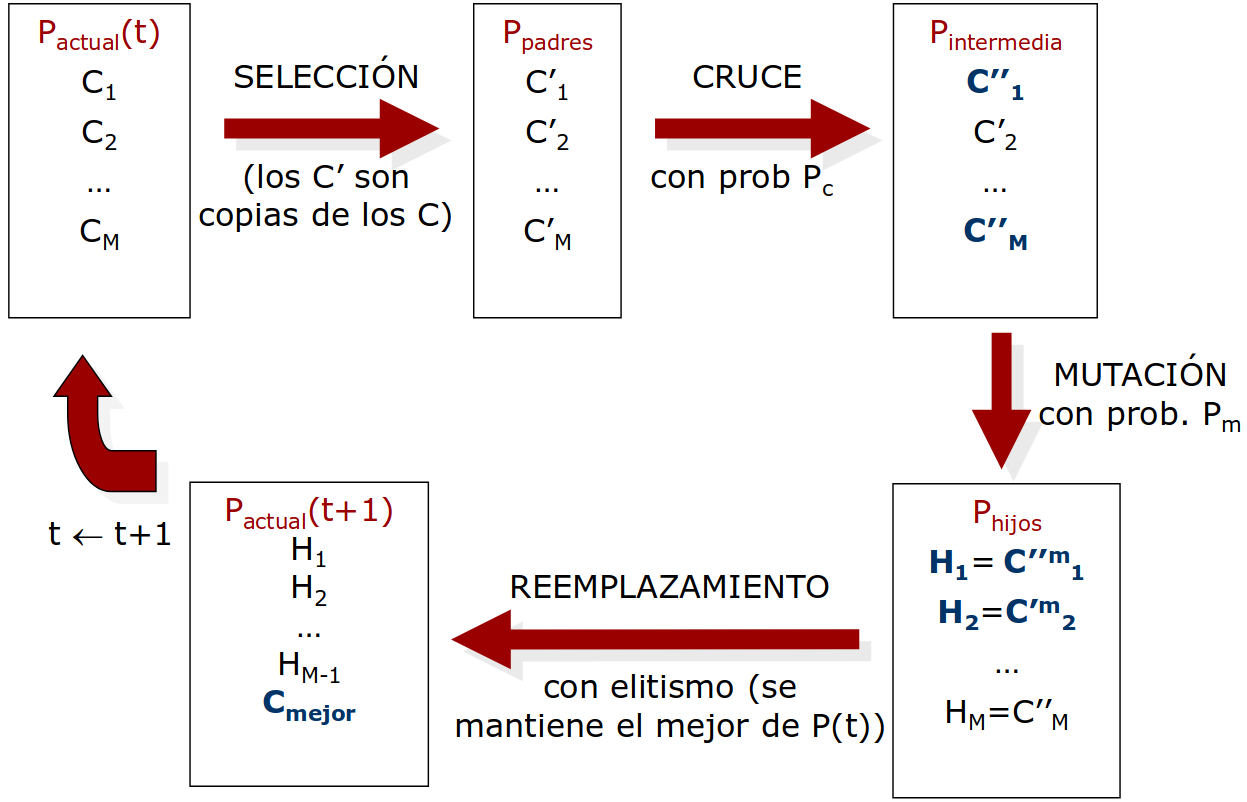
\includegraphics[scale=0.3]{esquema-agg}
      \end{center}
      
      
      Se ha desarrollado dos variantes elitistas: una con el operador de cruce basado en posición, y otra con el operador de cruce OX.\\
      
      Solo varían los operadores de selección y remplazo que se describen a continuación. El resto de operadores son los descritos anteriormente.
      
      \newpage
      \subsubsection*{Operador de Selección}
      Se usará un torneo binario, consistente en elegir aleatoriamente dos individuos de la población y seleccionar el mejor de ellos. Se aplicarán tantos torneos como individuos existan en la población.\\
      
      La implementación es la siguiente:\\
      \begin{algorithm}[H]
       	\caption{\textit{agg.cpp} - AGG::Select}
       	
         \SetKwProg{Def}{def}{:}{end}
         \Def{Select($P$)}{
         	\For{$i = 1$ \KwTo $n$}{
				$r1 = $ random in $[0, n)$\\
            	$r2 = $ random in $[0, n)$\\        	
         	
         		\If{coste $P_{r1}$ desconocido}{
            		Calcula coste $P_{r1}$\\
            		evaluaciones++\\
            	}
            	\If{coste $P_{r2}$ desconocido}{
            		Calcula coste $P_{r2}$\\
            		evaluaciones++\\
            	}
            	
            	\If{coste $P_{r1} \leq P_{r2}$}{
            		$P'_i = P_{r1}$\\
            	} \Else {
					$P'_i = P_{r2}$\\
            	}
         	}
                    
            
            \textbf{return} $P'$\\
         }
      \end{algorithm}
      
      
      \newpage
      \subsubsection*{Operador de Remplazo}
      Se remplaza la anterior población por la nueva remplazando la peor solución de esta por la mejor de la generación anterior. El pseudocódigo que implementa dicha funcionalidad es:\\
      
      \begin{algorithm}[H]
       	\caption{\textit{agg.cpp} - AGG::Replace}
       	
         \SetKwProg{Def}{def}{:}{end}
         \Def{Replace($P, P'$)}{
         	$P'' = P'$\\
         	$peor\_coste = peor\_indice = 0$\\
         	
         	\If{$\exists \pi_{best}$}{
         		\For{$i = 1$ \KwTo $n$}{      	
         	
         			\If{coste $P''_i$ desconocido}{
            			Calcula coste $P''_i$\\
            			evaluaciones++\\
            		}
            		\If{$peor\_coste < coste P''_i$}{
            			$peor\_coste = coste P''_i$\\
            			$peor\_indice = i$\\
            		}
         		}
         		
         		$P''_{peor\_indice} = \pi_{bestAnterior}$\\
         	}
                    
            
            \textbf{return} $P''$\\
         }
      \end{algorithm}
      
      
      
      
      
      
      \newpage
      \subsection{Algorítmo Genético Estacionario. \textit{AGE}}
      Durante cada iteración se escogen dos padres de la población y se les aplican los operadores genéticos. Este modelo es elitista. Además, produce una convergencia rápida ya que se remplazan los peores cromosomas de la población por los dos padres escogidos y modificados anteriormente, solo si estos mejoran a los peores de la población anterior.
      \begin{center}
      	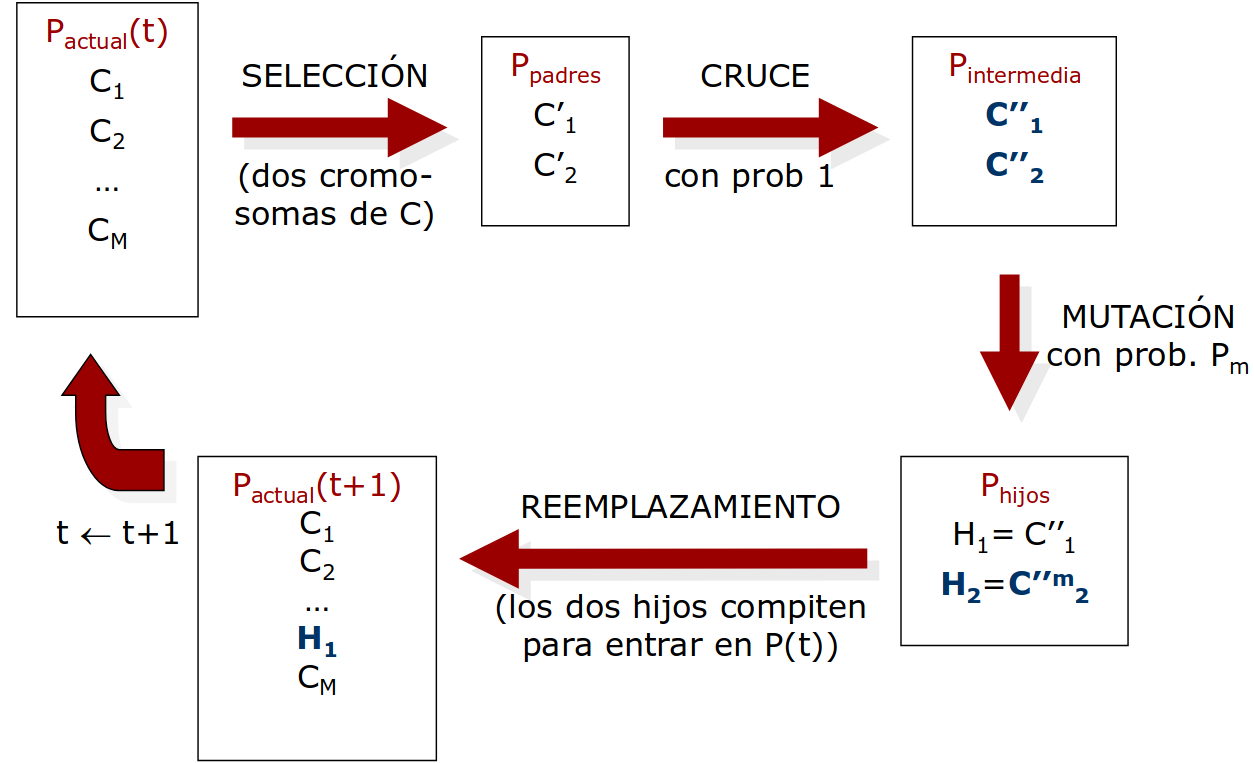
\includegraphics[scale=0.3]{esquema-age}
      \end{center}
      
      De nuevo, se han implementados dos variantes; una que utiliza un cruce basado en posición y otra en cruce OX.\\
      
      Al igual que en el AGG, solo cambian los operadores de selección y remplazo. No obstante notese que los padres escogidos siempre cruzan ya que la probabilidad de cruce es 1 en los AGE.
      
      \newpage
      \subsubsection*{Operador de Selección}
      De nuevo se utiliza un torneo binario. Se aplicarán 2 torneos para escoger dos padres con los que operar posteriormente.\\
      
      La implementación es la siguiente:\\
      
      \begin{algorithm}[H]
       	\caption{\textit{age.cpp} - AGE::Select}
       	
         \SetKwProg{Def}{def}{:}{end}
         \Def{Select($P$)}{
         	\For{$i = 1$ \KwTo $2$}{
				$r1 = $ random in $[0, n)$\\
            	$r2 = $ random in $[0, n)$\\        	
         	
         		\If{coste $P_{r1}$ desconocido}{
            		Calcula coste $P_{r1}$\\
            		evaluaciones++\\
            	}
            	\If{coste $P_{r2}$ desconocido}{
            		Calcula coste $P_{r2}$\\
            		evaluaciones++\\
            	}
            	
            	\If{coste $P_{r1} \leq P_{r2}$}{
            		$P'_i = P_{r1}$\\
            	} \Else {
					$P'_i = P_{r2}$\\
            	}
         	}
                    
            
            \textbf{return} $P'$\\
         }
      \end{algorithm}
      
      \newpage
      \subsubsection*{Operador de Remplazo}
      Se remplazan los (dos) peores cromosomas de la población original por los cromosomas de la nueva población solo si los segundos mejoran los primeros.\\
      
      Partiendo de una implementación básica con complejidad temporal $O(n^2)$; De nuevo se ha conseguido una implementación que sacrificando espacio consigue una eficiencia $O(n)$. \\
      
      La representación en pseudocódigo de este operador es la siguiente:\\
      
      \begin{algorithm}[H]
       	\caption{\textit{age.cpp} - AGE::Replace}
       	
         \SetKwProg{Def}{def}{:}{end}
         \Def{Replace($P, P'$)}{
         	$P'' = P$\\
         	$peores = set()$ \# Se ordenan los valores en función del coste\\
         	
         	\For{$i = 1$ \KwTo $len(P'')$}{
         		\If{coste $P''_i$ desconocido}{
            		Calcula coste $P''_i$\\
            		evaluaciones++\\
            	}
            	
            	\If{$peores == \O$ \textbf{or} $coste P''_i > coste peores_0$}{
            		\If{$len(peores) \geq len(P')$}{
            			Elimina $peores_0$ de $peores$\\ 
            		}
            		
            		$peores = peores \cup P''_i$
            	}
         	}
         	
         	\For{$i = 1$ \KwTo $len(P')$}{
         		\If{coste $P'_i$ desconocido}{
            		Calcula coste $P'_i$\\
            		evaluaciones++\\
            	}
            	
            	\For{$j = 1$ \KwTo $len(peores)$}{
            		\If{coste $peores_j >$ coste $P'_i$}{
            			cambiar el cromosoma $peores_j$ de $P''$ por $P_i$\\
            			eliminar $peores_j$ de $peores$\\
            		}
            	}
         	}
                    
            
            \textbf{return} $P''$\\
         }
      \end{algorithm}
      
      
      
      
      \newpage
      \section{Algorítmos Meméticos}
      Partiremos de un AGG con operador de cruce basado en posición sobre el cual, pasado un determinado número de iteraciones ($blN$), ejecutaremos una búsqueda local sobre un número de elementos calculado a partir de una probabilidad $P_{bl}$ y el tamaño de la población como:\\
      $$blExecN = \lceil P_{bl} \cdot n \rceil$$
      
      La búsqueda local se detiene cuando sobre un cromosoma no se ha encontrado un vecino mejor, cuando se explora todo el entorno sin encontrar una solucion mejor, o bien, cuando se alcanza un número máximo de evaluaciones sobre vecinos.\\
      	
      Gracias a esta hibridación de tecnicas, tenemos la ventaja de alcanzar rapidamente un óptimo local gracias a la búsqueda local, y la capacidad de aceptar soluciones peores como válidas a fin de evitar quedarnos atrapados en óptimos locales.\\
      
      Además, podemos elegir si aplicar la búsqueda local sobre los mejores de la población.\\
      
      \newpage
      La única función que cambia respecto a un algorítmo génetico es el método de búsqueda, cuya implementación es la siguiente:\\
      
      \begin{algorithm}[H]
       	\caption{\textit{memetic.cpp} - MemeticAlg::Solve}
       	
         \SetKwProg{Def}{def}{:}{end}
         \Def{Solve()}{
         	$P = GenerateRandomPopulation()$\\
         	$\pi = Evaluate(P)$;\hspace*{0.5cm}$\pi_{best} = \pi$;\hspace*{0.5cm}$generations = 0$\\
            \While{evaluaciones $\neq$ limite}{
            	$P' = Select(P)$\\
            	$P' = Cross(P')$\\
            	$P' = Mutate(P')$\\
            	$P' = Replace(P, P')$\\
            	
				\If{$generations == blN$}{
					$generations = 0$\\
				
					\If{aplicar en los mejores}{
						$P'' = P$\\
						Ordena los cromosomas de $P''$ con el coste de cada uno\\
						
						\For{$i=0$ \KwTo $blExecN$}{
							$\pi' = BusquedaLocalSobre(P''_i)$\\
							
							\lIf{$\exists \pi'$}{
								$P''_i = \pi'$
							}
						}
						
						Remplaza los modificados en $P''$ en $P'$\\
				
					} \Else {
						\For{$i=0$ \KwTo $blExecN$}{
							$\pi' = BusquedaLocalSobre(P'_i)$\\
							
							\lIf{$\exists \pi'$}{
								$P'_i = \pi'$
							}
						}					
					}
				
				
				}            	
            	
            	$\pi = Evaluate(P)$\\
            	
            	\lIf{$\pi$ mejor que $\pi_{best}$}{
            		$\pi_{best} = \pi$
            	}
            }         
            
            \textbf{return} $\pi_{best}$\\
         }
      \end{algorithm}
      
     	\newpage
     	\section{Enfriamiento Simulado}
     	El Enfriamiento simulado es un algoritmo de búsqueda por entornos con un criterio probabilístico de aceptación de soluciones basado en Termodinámica. Con el fin de evitar que el algoritmo termine en un óptimo local como en la Búsqueda Local, se permiten movimientos hacia soluciones peores.\\
     	
     	Sin embargo, esto debe hacerse de una manera controlada. En el enfriamiento simulado esto se realiza controlando la frecuencias con la que aceptamos soluciones perores a la actual mediante una función de probabilidad que hará disminuir la probabilidad de dichos movimientos. Es decir, primero diversificamos para luego finalmente intensificar la búsqueda. Sus funciones claves son las siguientes:
     	\begin{itemize}
     		\item \textbf{Operador de vecino:} Para crear un vecino aleatorio a partir de la solución actual, se intercambian dos posiciones de la representación de la solución aleatoriamente.
     		
     		\item \textbf{Temperatura inicial:} Se calculará en función de la siguiente fórmula.
     		$$T_{o} = \frac{\mu C(S_o)}{-ln(\phi)}$$
     		
     		Donde $T_o$ es la temperatura inicial, $C(S_o)$ el coste de la solución inicial, y $\phi \in [0,1]$ es la probabilidad de aceptar una solución un $\mu$ por 1 peor que la inicial. También se ha experimentado con un esquema proporcional dado por $T_{k+1} = \alpha T_k$ donde $\alpha \in [0.9, 0.99]$
     		
     		\item \textbf{Esquema de enfriamiento:} Se empleará el esquema de Cauchy modificado.
     		$$T_{k+1} = \frac{T_k}{1 + \beta T_k} \quad \quad \quad \beta = \frac{T_o - T_f}{MT_oT_f}$$
     		
     		Donde $M$ es el número de enfriamientos a realizar ($ \frac{\text{n maximo de evaluaciones}}{\text{n maximo de vecinos}}$), $T_o$ es la temperatura inicial y $T_f$ es la temperatura final cuyo valor será cercano a 0.
     		
     		\item \textbf{Condición de enfriamiento L(T):} Se enfría la temperatura bien cuando se genere un número máximo de vecinos, o cuando se acepte un número máximo de los vecinos generados.
     		
     		\item \textbf{Condición de parada:} Cuando se alcance un número máximo de iteraciones o cuando el número de éxitos en el enfriamiento actual sea 0.
     	\end{itemize}
     	
     	Todo las funciones anteriores se combinan para implementar el algoritmo que parte de una solución creada aleatoriamente como se explicó en la búsqueda local de la siguiente manera:\\
     	\begin{algorithm}[H]
       	\caption{\textit{simAnealing.cpp} - SimulatedAnealing::Solve}
       	
         \SetKwProg{Def}{def}{:}{end}
         \Def{Solve}{
         	$\pi$ = $\pi_{best}$ = GenerateRandomSolution()\\
         	$T = \frac{\mu C(\pi)}{-ln(\phi)} \quad \quad \beta = \frac{T - T_f}{MT_oT_f}$ \\
         	evals = 0\\
         	
         	\Do{$evals \leq maxEvals$ \textbf{and} $successes > 0$}{
               successes = neighGenerated = 0\\
               
               \While{$neighGenerated \leq maxNeighbours$ \textbf{and} $successes \leq maxSuccess$}{
               		$\pi'$ = intercambia dos posiciones (r, s) aleatorias de $\pi$\\
               		Calcular coste de $pi'$ con $\Delta C(\pi,r,s)$ \\
               		$neighGenerated = neighGenerated + 1$\\
               		$evals = evals + 1$\\
               		
               		\If{$C(\pi') < C(\pi)$ \textbf{or} $U(0,1) \leq e^{C(\pi,r,s)/T}$ }{
               			$\pi = \pi'$;\quad$successes = successes + 1$\\
               			
               			\If{$C(\pi) < C(\pi_{best})$}{
               				$\pi_{best} = \pi$\\
               			}
               		}
               }
               
               $T = \frac{T}{1 + \beta T}$\\
             }
             
             \textbf{return} $\pi_{best}$\\
         }
      \end{algorithm}
     	
     	
     	
     	
     	\newpage
     	\section{Búsqueda Multiarranque Básica}
     	Este algoritmo es muy sencillo, se basa en crear $n$ soluciones aleatorias a las que aplicar una búsqueda local y devolver la mejor solución obtenida. Dichas soluciones aleatorias se crean como se describió en la Búsqueda Local.\\
     	
     	A continuación se muestra el pseudocódigo que implementa este algoritmo:\\
     	\begin{algorithm}[H]
       	\caption{\textit{multistart.cpp} - MultiStartSearch::Solve}
       	
         \SetKwProg{Def}{def}{:}{end}
         \Def{Solve}{
         	$\pi_{best} = \emptyset$ \\
         	
         	\For{$i=1$ \KwTo $n$}{
         		$\pi$ = GenerateRandomSolution()\\
         		$\pi$ = aplicar busqueda local sobre $\pi$\\
         		
         		\If{$\pi_{best} == \emptyset$ \textbf{or} $C(\pi) < C(\pi_{best})$}{
         			$\pi_{best} = \pi$\\
         		}
         	}
         	
         	\textbf{return} $\pi_{best}$\\
         }
      \end{algorithm}
     	
     	
     	\newpage
     	\section{GRASP}
     	Un algoritmo GRASP es un método multiarranque, en el que cada iteración consiste en la construcción de una solución greedy aleatorizada y la aplicación de una búsqueda local que toma dicha solución como punto inicial de la búsqueda.\\
     	
     	Este procedimiento se repite varias veces y la mejor solución encontrada sobre todas las iteraciones GRASP se devuelve como salida del algoritmo. Para ilustrar este comportamiento se ha compuesto el siguiente pseudocódigo:\\
     	\begin{algorithm}[H]
       	\caption{\textit{grasp.cpp} - GRASP::Solve}
       	
         \SetKwProg{Def}{def}{:}{end}
         \Def{Solve}{
         	$\pi_{best} = \emptyset$ \\
         	
         	\For{$i=1$ \KwTo $n$}{
         		$\pi$ = GenerateRandomGreedySolution()\\
         		$\pi$ = aplicar busqueda local sobre $\pi$\\
         		
         		\If{$\pi_{best} == \emptyset$ \textbf{or} $C(\pi) < C(\pi_{best})$}{
         			$\pi_{best} = \pi$\\
         		}
         	}
         	
         	\textbf{return} $\pi_{best}$\\
         }
      \end{algorithm}
     	
     	\newpage
     	\subsection{Algoritmo Greedy Aleatoreizado}
     	Es necesario explicar como funciona el greedy aleatorizado para el problema del QAP, pues su implementación no es la misma que la del greedy común.\\
     	
     	En cada iteración de su proceso constructivo de la solución, se construye una lista de candidatos factibles la cual se acota con un tamaño variable en función de un umbral de calidad. El elemento seleccionado se escoge aleatoriamente de esta lista acotada. Dicha cota se calcula como:
     	\begin{itemize}
     		\item \textbf{Para las unidades:} $\mu = d_{max} - \alpha(d_{max}-d_{min})$. Donde donde $d_{max}$ es el mayor valor de flujo potencial de los candidatos y $d_{min}$ el menor.
     		
     		\item \textbf{Para las localizaciones:} $\mu = d_{min} + \alpha(d_{max}-d_{min})$.
     	\end{itemize}
     	
     	 Se pueden diferenciar dos etapas del proceso de creación de la solución:
     	\begin{enumerate}
     		\item Se asignan conjuntamente dos unidades a dos localizaciones. Se consideran los potenciales de flujo y distancia para escoger el par de asignaciones.
     		
     		\item Se toman las n-2 decisiones restantes asignando una unidad a una localización en cada paso. Se escoge la asignación factible con el mínimo coste de interacción con respecto a las asignaciones realizadas hasta ahora de acuerdo a una decisión greedy aleatorizada.
     	\end{enumerate}
     	
     	A continuación se expone un pseudocódigo que lleva esto acabo:\\
     	\begin{algorithm}[H]
       	\caption{\textit{grasp.cpp} - RandomGreedy::Solve}
       	
         \SetKwProg{Def}{def}{:}{end}
         \Def{Solve}{
         	clFrequencies = vector de parejas ($u_i$, $\hat{f}_i$)\\
         	clDistances = vector de parejas ($l_i$, $\hat{d}_i$)\\
         	unitAsigned = bool vector[len(clFrequencies)]\{0\}\\
         	locAsigned = bool vector[len(clDistances)]\{0\}\\
         	$\pi_p = \emptyset$\\
         	
         	\vspace*{0.1cm}
         	ordenar clFrequencies por $\hat{f}_i$;\hspace*{0.2cm} ordenar clDistances por $\hat{d}_i$\\
         	
         	\vspace*{0.1cm}
         	$\mu_u = clFrequencies_n - \alpha(clFrequencies_n - clFrequencies_0)$\\
         	$\mu_l = clDistances_0 + \alpha(clDistances_n - clDistances_0)$\\
         	
         	\vspace*{0.1cm}
         	$i_u$ = buscar el primer elemento que supera $\mu_u$\\
         	$i_l$ = buscar el primer elemento que supera $\mu_l$\\
         	
         	\vspace*{0.1cm}
         	$rnd_{u_1} = U(i_u, n)$; $\quad rnd_{l_1} = U(0, l_u)$\\
         	$rnd_{u_2} = U(i_u, n) | rnd_{u_1} \neq rnd_{u_2}$; \hspace*{0.2cm}$rnd_{l_2} = U(0, l) | rnd_{l_1} \neq rnd_{l_2}$\\
         	
         	$\pi_p = \pi_p \cup (clFrequencies_{rnd_{u_{1_0}}}, clDistancess_{rnd_{l_{1_0}}})$\\
         	$\pi_p = \pi_p \cup (clFrequencies_{rnd_{u_{2_0}}}, clDistancess_{rnd_{l_{2_0}}})$\\
         	$unitAsigned_{clFrequencies_{rnd_{u_{1_0}}}} = unitAsigned_{clFrequencies_{rnd_{u_{2_0}}}} = 1$\\
         	$locAsigned_{clDistances_{rnd_{l_{1_0}}}} = locAsigned_{clDistances_{rnd_{l_{2_0}}}} = 1$\\
         	
         	
         	\For{$i=3$ \KwTo $len(clFrequencies)$}{
         		$bestCost = \inf$; \hspace*{0.2cm} $bestPair = \emptyset$\\
         		\For{$u=1$ \KwTo $len(clFrequencies)$}{
         			\lIf{$unitAssigned_u == 1$}{\textbf{continue}}
         			
         			\For{$l=1$ \KwTo $len(clDistances)$}{
         				\lIf{$locAssigned_l == 1$}{\textbf{continue}}
         				
         				$cost = \sum_{(j, k) \in \pi_p} f_{uj}d_{lk}$\\
         				
         				\If{$cost < bestCost$}{
         					$bestCost = cost$\\
         					$bestpair = (u, l)$\\
         				}
         			
         			}
         		}
         		
         		$\pi_p = \pi_p \cup bestPair$\\
         		$unitAsigned_{bestPair_0} = locAsigned_{bestPair_1} = 1$\\
         	}
         	
         	$\pi = $ solucion del tamaño de la solución parcial\\
         	\For{$i=0$ \KwTo $len(\pi_p)$}{
         		$\pi(\pi_{p_{i_0}}) = \pi_{p_{i_1}}$\\
         	}
         	
         	\textbf{return} $\pi$\\
         }
      \end{algorithm}

     	\newpage
     	\section{Búsqueda Local Reiterada}
     	También conocido como ILS (Iterated Local Search), está basado en la aplicación repetida de una búsqueda local sobre una solución inicial que se obtiene por mutación de un óptimo local previamente encontrado.\\
     	
     	Como operador de mutación usaremos el operador de vecino de sublista aleatoria de tamaño fijo t. Este consiste en seleccionar una cadena de asignaciones de tamaño t y barajarlas. Haremos que t sea un cuarto del tamaño de la solución para provocar cambios bruscos.\\
     	\begin{algorithm}[H]
       	\caption{\textit{ils.cpp} - ILS::Mutate}
       	
         \SetKwProg{Def}{def}{:}{end}
         \Def{Mutate($\pi_o$)}{
         	$sliceSize = \lceil 0.4 \cdot len(\pi_o) \rceil$\\
         	$start = U(0, len(\pi_o) - sliceSize)$\\
         	$end = start + sliceSize$\\
         	$\pi' = \pi$\\
         	
         	barajar las localizacion desde $\pi'(start)$ a $\pi'(end)$
         	
         	\textbf{return} $\pi'$\\
         }
      \end{algorithm}
      
      El pseudocódigo que ilustra el funcionamiento general de ILS es el siguiente:\\
      \begin{algorithm}[H]
       	\caption{\textit{ILS.cpp} - ILS::Solve}
       	
         \SetKwProg{Def}{def}{:}{end}
         \Def{Solve}{
         	$\pi_{best} = GenerateRandomsolution()$ \\
         	$\pi_{best} = $ aplicar búsqueda local sobre $\pi_{best}$\\
         	
         	\For{$i=2$ \KwTo $n$}{
         		$\pi$ = Mutar $\pi_{best}$\\
         		$\pi$ = aplicar búsqueda local sobre $\pi$\\
         		
         		\If{$C(\pi) < C(\pi_{best})$}{
         			$\pi_{best} = \pi$\\
         		}
         	}
         	
         	\textbf{return} $\pi_{best}$\\
         }
      \end{algorithm}
      
     	
     	\subsection{Hibridación con Enfriamiento Simulado}
     	Exactamente igual que el ILS clásico pero substituyendo la búsqueda local por un enfriamiento simulado.
      
      
      \newpage
      \section{Procedimiento considerado para desarrollar la práctica}
      Esta práctica ha sido desarrollada en \textbf{C++} como una librería de metaheurísticas. La estructura del proyecto es la siguiente:\\
      
      \dirtree{%
         .1 /Software.
         .2 bin/         \DTcomment{Archivos ejecutables}.
         .3 practica1   \DTcomment{Ejecutable principal de la práctica}.
         .2 build/       \DTcomment{Directorio para compilación con CMake}.
         .2 doc/         \DTcomment{Otra documentación y código LaTeX de este documento}.
         .2 include/     \DTcomment{Cabeceras}.
         .2 instancias/  \DTcomment{Instancias de problemas sobre QAP}.
         .3 *.dat   \DTcomment{Definición de un problema}.
         .3 *.sln   \DTcomment{Solución a un problema}.
         .2 src/         \DTcomment{Código fuente}.
         .2 CMakeLists.txt   \DTcomment{Instrucciones de compilación para CMake}.
         .2 readme.txt       \DTcomment{Instrucciones de uso}.
      }\vspace*{0.5cm}
      
      Para compilar este proyecto necesitamos las herramientas \textit{g++} y \textit{CMake}. Para instalarlas en un sistema \textbf{Ubuntu} o derivado, ejecutamos:
      
      \begin{lstlisting}[language=bash]
      sudo apt-get install g++ cmake 
      \end{lstlisting}
      
      Podemos compilar el proyecto con dos niveles de optimización:
      \begin{itemize}
         \item \textbf{Debug}: Sin optimización y con símbolos de depuración. Ejecutar CMake con opción \textit{-D CMAKE\_BUILD\_TYPE=Debug}
         
         \item \textbf{Release}: Máxima optimización en la compilación. Por defecto.
      \end{itemize}
      
      Se compila con las siguientes instrucciones:
      
      \begin{lstlisting}[language=bash]
   cd build/
   # Para debug: cmake -D CMAKE_BUILD_TYPE=Debug ..
   cmake ..  
   make clean
   make
   cd ..
      \end{lstlisting}
      
      \newpage
      La sintaxis de ejecución es la siguiente\footnote{El parámetro semilla es opcional, por defecto $semilla = 7$}:
      \begin{lstlisting}[language=bash]
./bin/main instancias/<problema>.dat <semilla>
      \end{lstlisting}
      
      Por ejemplo:
      \begin{lstlisting}[language=bash]
./bin/main instancias/chr22a.dat 12
      \end{lstlisting}
      
      La salida del programa tiene la siguiente estructura:
      \begin{center}
      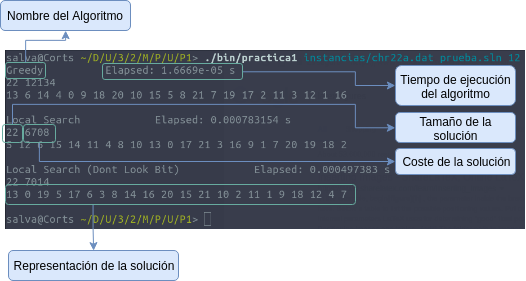
\includegraphics[scale=0.7]{execOutDiagram}
      \end{center}
      
      
      \newpage
      \section{Experimentos y análisis de resultados}
      Con el fin de comparar los algoritmos implementados con los ya existentes, vamos a calcular para cada algoritmo los siguientes parámetros:
      \begin{itemize}
         \item \textbf{\textit{Desv}}: Media de las desviaciones en porcentaje, del valor obtenido por cada método en cada instancia respecto al mejor valor conocido para ese caso.
         $$ \frac{1}{\left | casos \right |}\sum_{i=1}^{casos}100\frac{valoralgoritmo_i - mejorValor_i}{mejorValor_i} $$
         Obtendremos los mejores valores conocidos de \textit{QAPLIB}\footnote{http://anjos.mgi.polymtl.ca/qaplib//inst.html}
         
         \item \textbf{\textit{Tiempo}}: se calcula como la media del tiempo de ejecución empleado por el
algoritmo para resolver cada caso del problema.
      \end{itemize}
      
      Cuanto menor es el valor de Desv para un algoritmo, mejor calidad tiene dicho algoritmo. Por otro lado, si dos métodos obtienen soluciones de la misma calidad (tienen valores de Desv similares), uno será mejor que el otro si emplea menos tiempo en media.\\
      
\emph{\textbf{Parámetros del experimento:} 
   \begin{itemize}
      \item El valor de la semilla para este experimento es 7.
      \item Se compilara con parámetro \textbf{debug} a fin de contrastar aún mas los resultados del tiempo entre los algorimos greedy y búsqueda local.
      \item Los tiempos para los algoŕimos genéticos y meméticos se han tomado con compilación \textbf{Release}, por lo tanto, se compará con el tiempo medio del greedy y búsqueda local compilados en \textbf{Release}.
   \end{itemize}
}      

      
      \newpage
      \subsection{Resultados Greedy}
\begin{table}[H]
\centering
\label{my-label}
\begin{tabular}{|l|l|l|l|l|l|l|}
\hline
\multicolumn{7}{|c|}{\textbf{Algoritmo Greedy}}                                                                                                                                                \\ \hline
\textbf{Caso}    & \multicolumn{1}{c|}{\textbf{Desv}} & \multicolumn{1}{c|}{\textbf{Tiempo}} &  & \textbf{Caso}    & \multicolumn{1}{c|}{\textbf{Desv}} & \multicolumn{1}{c|}{\textbf{Tiempo}} \\ \cline{1-3} \cline{5-7} 
\textbf{Chr22a}  & 97,11                              & 0,000126925                          &  & \textbf{Sko100a} & 13,36                              & 0,000630563                          \\ \cline{1-3} \cline{5-7} 
\textbf{Chr22b}  & 134,48                             & 0,000125567                          &  & \textbf{Sko100f} & 13,77                              & 0,00230857                           \\ \cline{1-3} \cline{5-7} 
\textbf{Chr25a}  & 448,47                             & 0,000175691                          &  & \textbf{Tai100a} & 13,80                              & 0,000616869                          \\ \cline{1-3} \cline{5-7} 
\textbf{Esc128}  & 140,63                             & 0,00117301                           &  & \textbf{Tai100b} & 32,79                              & 0,000626035                          \\ \cline{1-3} \cline{5-7} 
\textbf{Had20}   & 7,71                               & 0,000102693                          &  & \textbf{Tai150b} & 24,97                              & 0,00136394                           \\ \cline{1-3} \cline{5-7} 
\textbf{Lipa60b} & 27,59                              & 0,000289296                          &  & \textbf{Tai256c} & 120,48                             & 0,00340613                           \\ \cline{1-3} \cline{5-7} 
\textbf{Lipa80b} & 28,58                              & 0,000382927                          &  & \textbf{Tho40}   & 29,96                              & 0,000384573                          \\ \cline{1-3} \cline{5-7} 
\textbf{Nug28}   & 22,88                              & 0,00020704                           &  & \textbf{Tho150}  & 16,98                              & 0,00204635                           \\ \cline{1-3} \cline{5-7} 
\textbf{Sko81}   & 15,50                              & 0,0013694                            &  & \textbf{Wil50}   & 11,68                              & 0,00017995                           \\ \cline{1-3} \cline{5-7} 
\textbf{Sko90}   & 13,61                              & 0,00162198                           &  & \textbf{Wil100}  & 7,33                               & 0,000619954                          \\ \cline{1-3} \cline{5-7} 
\end{tabular}
\end{table}

      Como podríamos esperar, el algoritmo greedy es muy rápido, aunque las soluciones obtenidas distan bastante de la mejor conocida. Podríamos discutir su utilidad desde un punto de vista práctico; ¿En qué escenarios puede sernos útil una búsqueda greedy?
      
      \begin{enumerate}
         \item Si ofrecemos un servicio donde la optimalidad de la solución a un problema es lo de menos y tenemos que responder muchas solicitudes con pocos recursos de manera muy rápida.
         
         \item Como algoritmo auxiliar de cara a obtener una solución inicial para posteriormente tratar de mejorarla mediante el uso de algoritmos mas complejos. No obstante, esto no siempre es buena idea pues corremos el riesgo de caer en óptimos locales. Hay que usarlos con algoritmos que sean capaces de esquivar con relativa facilidad óptimos locales.         
      \end{enumerate}
      
      \begin{center}
         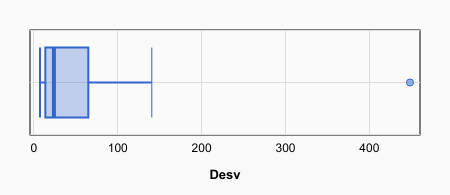
\includegraphics[scale=0.42]{boxplot-greedy-desv}
         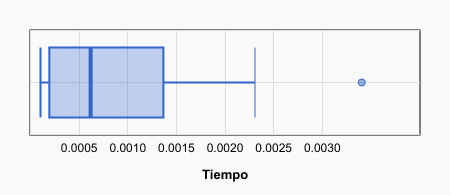
\includegraphics[scale=0.42]{boxplot-greedy-time}
      \end{center}
      
      
      \newpage
      \subsection{Resultados Búsqueda Local}
\begin{table}[H]
\centering
\label{my-label}
\begin{tabular}{|l|l|l|l|l|l|l|}
\hline
\multicolumn{7}{|c|}{\textbf{Algoritmo Búsqueda Local}}                                                                                                                                    \\ \hline
\textbf{Caso}    & \multicolumn{1}{c|}{\textbf{Desv}} & \multicolumn{1}{c|}{\textbf{Tiempo}} &  & \textbf{Caso}    & \multicolumn{1}{c|}{\textbf{Desv}} & \multicolumn{1}{c|}{\textbf{Tiempo}} \\ \cline{1-3} \cline{5-7} 
\textbf{Chr22a}  & 17,41                              & 0,00255601                           &  & \textbf{Sko100a} & 2,53                               & 1,54504                              \\ \cline{1-3} \cline{5-7} 
\textbf{Chr22b}  & 15,63                              & 0,00382979                           &  & \textbf{Sko100f} & 2,21                               & 2,05617                              \\ \cline{1-3} \cline{5-7} 
\textbf{Chr25a}  & 75,40                              & 0,00940898                           &  & \textbf{Tai100a} & 3,35                               & 0,806562                             \\ \cline{1-3} \cline{5-7} 
\textbf{Esc128}  & 18,75                              & 0,360157                             &  & \textbf{Tai100b} & 4,94                               & 3,26802                              \\ \cline{1-3} \cline{5-7} 
\textbf{Had20}   & 1,44                               & 0,0058809                            &  & \textbf{Tai150b} & 3,50                               & 24,8278                              \\ \cline{1-3} \cline{5-7} 
\textbf{Lipa60b} & 19,79                              & 0,114542                             &  & \textbf{Tai256c} & 1,26                               & 5,15624                              \\ \cline{1-3} \cline{5-7} 
\textbf{Lipa80b} & 22,30                              & 0,291904                             &  & \textbf{Tho40}   & 5,34                               & 0,0626425                            \\ \cline{1-3} \cline{5-7} 
\textbf{Nug28}   & 8,94                               & 0,0114589                            &  & \textbf{Tho150}  & 2,78                               & 13,1679                              \\ \cline{1-3} \cline{5-7} 
\textbf{Sko81}   & 2,70                               & 0,540895                             &  & \textbf{Wil50}   & 1,96                               & 0,10151                              \\ \cline{1-3} \cline{5-7} 
\textbf{Sko90}   & 1,86                               & 1,46495                              &  & \textbf{Wil100}  & 1,07                               & 2,19904                              \\ \cline{1-3} \cline{5-7} 
\end{tabular}
\end{table}

      Aunque no se obtienen soluciones óptimas, estas están muy cerca de serlo. Podemos apreciar que este algoritmo trabaja muy bien con problemas relativamente pequeños pero dado que, a diferencia del greedy, el tiempo crece significativamente en función del tamaño del problema, utilizarlo como algoritmo de propósito general para solucionar problemas no es lo idóneo.\\
      
      Sin embargo, en combinación con otros algoritmos como los Genéticos podemos obtener resultados aún mejores y en un tiempo mas aceptable dado que restringimos el espacio de búsqueda para este algoritmo.

      \begin{center}
         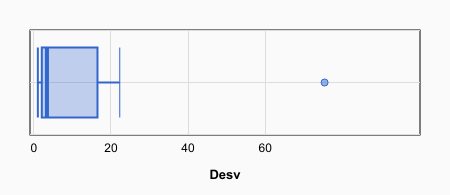
\includegraphics[scale=0.5]{boxplot-bl-desv}
         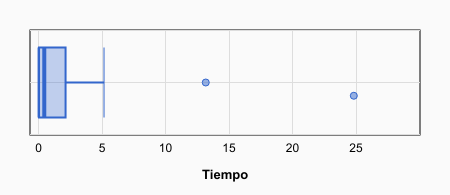
\includegraphics[scale=0.5]{boxplot-bl-time}
      \end{center}

      
      \newpage
      \subsection{Resultados Búsqueda Local con \textit{Don't Look Bits}}
\begin{table}[H]
\centering
\label{my-label}
\begin{tabular}{|l|l|l|l|l|l|l|}
\hline
\multicolumn{7}{|c|}{\textbf{Algoritmo Búsqueda Local DLB}}                                                                                                                                    \\ \hline
\textbf{Caso}    & \multicolumn{1}{c|}{\textbf{Desv}} & \multicolumn{1}{c|}{\textbf{Tiempo}} &  & \textbf{Caso}    & \multicolumn{1}{c|}{\textbf{Desv}} & \multicolumn{1}{c|}{\textbf{Tiempo}} \\ \cline{1-3} \cline{5-7} 
\textbf{Chr22a}  & 18.23                              & 0,0020404                            &  & \textbf{Sko100a} & 2.78                               & 0,229239                             \\ \cline{1-3} \cline{5-7} 
\textbf{Chr22b}  & 9.07                               & 0,0059782                            &  & \textbf{Sko100f} & 2.5                                & 0,226626                             \\ \cline{1-3} \cline{5-7} 
\textbf{Chr25a}  & 43.52                              & 0,00274717                           &  & \textbf{Tai100a} & 4.12                               & 0,164417                             \\ \cline{1-3} \cline{5-7} 
\textbf{Esc128}  & 12.5                               & 0,193508                             &  & \textbf{Tai100b} & 4.89                               & 0,418418                             \\ \cline{1-3} \cline{5-7} 
\textbf{Had20}   & 2.11                               & 0,00561109                           &  & \textbf{Tai150b} & 2.59                               & 1,5031                               \\ \cline{1-3} \cline{5-7} 
\textbf{Lipa60b} & 20.23                              & 0,0302634                            &  & \textbf{Tai256c} & 0.79                               & 1,84737                              \\ \cline{1-3} \cline{5-7} 
\textbf{Lipa80b} & 22.08                              & 0,0758918                            &  & \textbf{Tho40}   & 6.52                               & 0,0116882                            \\ \cline{1-3} \cline{5-7} 
\textbf{Nug28}   & 3.45                               & 0,0058682                            &  & \textbf{Tho150}  & 2.18                               & 1,14028                              \\ \cline{1-3} \cline{5-7} 
\textbf{Sko81}   & 2.1                                & 0,141866                             &  & \textbf{Wil50}   & 1.7                                & 0,0221609                            \\ \cline{1-3} \cline{5-7} 
\textbf{Sko90}   & 2.67                               & 0,246332                             &  & \textbf{Wil100}  & 1.26                               & 0,252535                             \\ \cline{1-3} \cline{5-7} 
\end{tabular}
\end{table}

      Podemos observar que la técnica de \textit{Don't look bits} mejora significativamente los tiempos de ejecución de la versión básica de la búsqueda local.
      
      \vspace*{1cm}
      \begin{center}
         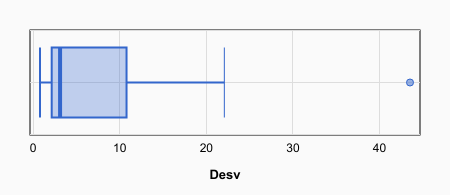
\includegraphics[scale=0.6]{boxplot-bldlb-desv}
         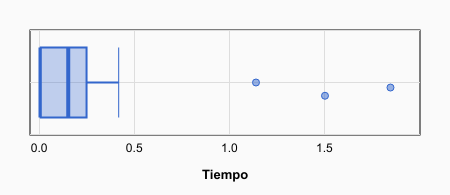
\includegraphics[scale=0.6]{boxplot-bldlb-time}
      \end{center}
      
      \newpage
         En el siguiente gráfico podemos ver como evoluciona el tiempo de ejecución en función del tamaño tanto de la Búsqueda Local (rojo) como de su variante con \textit{Don't Look Bits} (azul). \\
          
      \begin{center}
         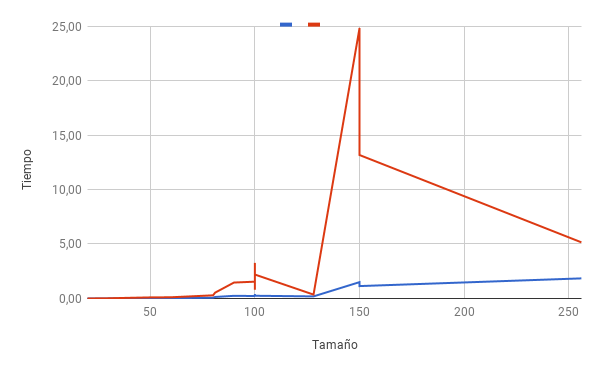
\includegraphics[scale=0.6]{bl-vs-dlb}
      \end{center}
      
      Se puede ver como el tamaño del problema no es lo único que afecta al tiempo de ejecución; La dificultad del problema en si (que es mucho mas difícil de medir) influye también. Por ejemplo, para la búsqueda local básica, se tarda más en \textit{Tai150b} de tamaño 150 (24,83 segundos) que en \textit{Tai256c} de tamaño 256 (5,15 segundos).
      
      \newpage
      \subsection{Resultados AGG con cruce basado en posición}
      \begin{table}[H]
\centering
\label{my-label}
\begin{tabular}{|l|l|l|l|l|l|l|}
\hline
\multicolumn{7}{|c|}{\textbf{Algoritmo AGG-Posición}}                                                                                                                                                       \\ \hline
\multicolumn{1}{|c|}{\textbf{Caso}} & \multicolumn{1}{c|}{\textbf{Desv}} & \multicolumn{1}{c|}{\textbf{Tiempo}} & \multicolumn{1}{c|}{} & \multicolumn{1}{c|}{\textbf{Caso}} & \multicolumn{1}{c|}{\textbf{Desv}} & \multicolumn{1}{c|}{\textbf{Tiempo}} \\ \cline{1-3} \cline{5-7} 
\textbf{Chr22a}                     & 11,86                     & 0,06                        &                       & \textbf{Sko100a}                   & 3,62                      & 0,61                        \\ \cline{1-3} \cline{5-7} 
Chr22b                     & 14,37                     & 0,06                        &                       & \textbf{Sko100f}                   & 3,36                      & 0,63                        \\ \cline{1-3} \cline{5-7} 
\textbf{Chr25a}                     & 52,85                     & 0,08                        &                       & \textbf{Tai100a}                   & 5,09                      & 0,60                        \\ \cline{1-3} \cline{5-7} 
\textbf{Esc128}                     & 40,63                     & 0,95                        &                       & \textbf{Tai100b}                   & 10,52                     & 0,63                        \\ \cline{1-3} \cline{5-7} 
\textbf{Had20}                      & 0,46                      & 0,06                        &                       & \textbf{Tai150b}                   & 12,81                     & 1,81                        \\ \cline{1-3} \cline{5-7} 
\textbf{Lipa60b}                    & 20,94                     & 0,24                        &                       & \textbf{Tai256c}                   & 3,63                      & 3,73                        \\ \cline{1-3} \cline{5-7} 
\textbf{Lipa80b}                    & 22,68                     & 0,42                        &                       & \textbf{Tho40}                     & 2,75                      & 0,14                        \\ \cline{1-3} \cline{5-7} 
\textbf{Nug28}                      & 5,92                      & 0,08                        &                       & \textbf{Tho150}                    & 7,22                      & 1,27                        \\ \cline{1-3} \cline{5-7} 
\textbf{Sko81}                      & 4,25                      & 0,40                        &                       & \textbf{Wil50}                     & 2,31                      & 0,20                        \\ \cline{1-3} \cline{5-7} 
\textbf{Sko90}                      & 3,47                      & 0,64                        &                       & \textbf{Wil100}                    & 2,30                      & 0,59                        \\ \cline{1-3} \cline{5-7} 
\end{tabular}
\end{table}

	Rápidamente obtenemos soluciones bastante buenas a nuestro problema. Aunque en las primeras iteraciones, este tipo de cruce genera hijos que se diferencian mas de los padres que los generados por el cruce OX, poco a poco, al ser un modelo elitista, la población converge hasta el punto de que muchos padres son iguales y por lo tanto, debido al funcionamiento de este tipo de cruce, los hijos son iguales. Todo esto hace que para pocas evaluaciones, este cruce actue mejor quer OX, pero un número lo suficientemente elevado de evaluaciones, el cruce basado en posición hará que la población se estanque y OX funcione mejor.

	\begin{center}
         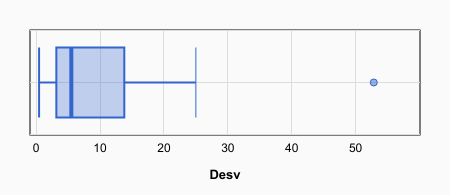
\includegraphics[scale=0.5]{boxplot-aggpos-desv}
         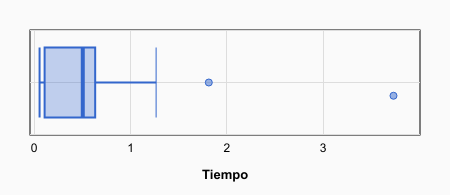
\includegraphics[scale=0.5]{boxplot-aggpos-time}
      \end{center}

		
	  \newpage
      \subsection{Resultados AGG con cruce OX}
      \begin{table}[H]
\centering
\label{my-label}
\begin{tabular}{|l|l|l|l|l|l|l|}
\hline
\multicolumn{7}{|c|}{\textbf{Algoritmo AGG-OX}}                                                                                                                                                             \\ \hline
\multicolumn{1}{|c|}{\textbf{Caso}} & \multicolumn{1}{c|}{\textbf{Desv}} & \multicolumn{1}{c|}{\textbf{Tiempo}} & \multicolumn{1}{c|}{} & \multicolumn{1}{c|}{\textbf{Caso}} & \multicolumn{1}{c|}{\textbf{Desv}} & \multicolumn{1}{c|}{\textbf{Tiempo}} \\ \cline{1-3} \cline{5-7} 
\textbf{Chr22a}                     & 34,73                     & 0,11                        &                       & \textbf{Sko100a}                   & 10,21                     & 0,90                        \\ \cline{1-3} \cline{5-7} 
\textbf{Chr22b}                     & 34,42                     & 0,11                        &                       & \textbf{Sko100f}                   & 11,52                     & 0,89                        \\ \cline{1-3} \cline{5-7} 
\textbf{Chr25a}                     & 142,41                    & 0,13                        &                       & \textbf{Tai100a}                   & 9,81                      & 0,88                        \\ \cline{1-3} \cline{5-7} 
\textbf{Esc128}                     & 109,38                    & 1,42                        &                       & \textbf{Tai100b}                   & 25,56                     & 0,91                        \\ \cline{1-3} \cline{5-7} 
\textbf{Had20}                      & 3,24                      & 0,13                        &                       & \textbf{Tai150b}                   & 19,43                     & 1,64                        \\ \cline{1-3} \cline{5-7} 
\textbf{Lipa60b}                    & 25,54                     & 0,48                        &                       & \textbf{Tai256c}                   & 4,85                      & 3,81                        \\ \cline{1-3} \cline{5-7} 
\textbf{Lipa80b}                    & 25,98                     & 0,66                        &                       & \textbf{Tho40}                     & 16,97                     & 0,25                        \\ \cline{1-3} \cline{5-7} 
\textbf{Nug28}                      & 11,73                     & 0,15                        &                       & \textbf{Tho150}                    & 13,65                     & 1,63                        \\ \cline{1-3} \cline{5-7} 
\textbf{Sko81}                      & 10,78                     & 0,68                        &                       & \textbf{Wil50}                     & 7,32                      & 0,33                        \\ \cline{1-3} \cline{5-7} 
\textbf{Sko90}                      & 11,14                     & 0,76                        &                       & \textbf{Wil100}                    & 6,50                      & 0,89                        \\ \cline{1-3} \cline{5-7} 
\end{tabular}
\end{table}

	Como hemos comentado antes, para un número de evaluaciones máximas pequeño, OX funciona peor que el cruce basado en posición. Sin embargo, trada más en converger.\\

	\begin{center}
         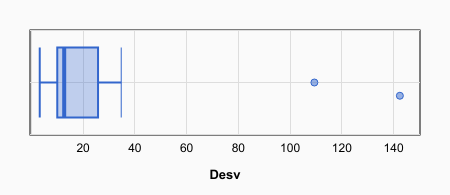
\includegraphics[scale=0.5]{boxplot-aggox-desv}
         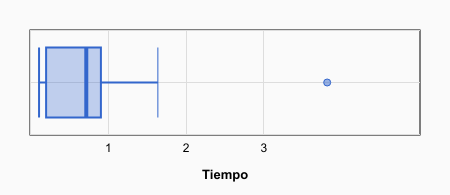
\includegraphics[scale=0.5]{boxplot-aggox-time}
      \end{center}
      
      
      \newpage
      \subsection{Resultados AGE con cruce basado en posición}
      \begin{table}[H]
\centering
\label{my-label}
\begin{tabular}{|l|l|l|l|l|l|l|}
\hline
\multicolumn{7}{|c|}{\textbf{Algoritmo AGE-Posición}}                                                                                                                                                                                                                   \\ \hline
\multicolumn{1}{|c|}{\textbf{Caso}} & \multicolumn{1}{c|}{\textbf{Desv}} & \multicolumn{1}{c|}{\textbf{Tiempo}} & \multicolumn{1}{c|}{\textbf{}} & \multicolumn{1}{c|}{\textbf{Caso}} & \multicolumn{1}{c|}{\textbf{Desv}} & \multicolumn{1}{c|}{\textbf{Tiempo}} \\ \cline{1-3} \cline{5-7} 
\textbf{Chr22a}                     & 14,78                              & 0,09                                 &                                & \textbf{Sko100a}                   & 3,07                               & 0,63                                 \\ \cline{1-3} \cline{5-7} 
\textbf{Chr22b}                     & 14,40                              & 0,07                                 &                                & \textbf{Sko100f}                   & 3,63                               & 0,60                                 \\ \cline{1-3} \cline{5-7} 
\textbf{Chr25a}                     & 48,52                              & 0,08                                 &                                & \textbf{Tai100a}                   & 4,57                               & 0,51                                 \\ \cline{1-3} \cline{5-7} 
\textbf{Esc128}                     & 28,13                              & 0,86                                 &                                & \textbf{Tai100b}                   & 10,50                              & 0,51                                 \\ \cline{1-3} \cline{5-7} 
\textbf{Had20}                      & 0,72                               & 0,08                                 &                                & \textbf{Tai150b}                   & 6,42                               & 1,02                                 \\ \cline{1-3} \cline{5-7} 
\textbf{Lipa60b}                    & 20,38                              & 0,28                                 &                                & \textbf{Tai256c}                   & 1,98                               & 3,13                                 \\ \cline{1-3} \cline{5-7} 
\textbf{Lipa80b}                    & 21,90                              & 0,46                                 &                                & \textbf{Tho40}                     & 5,08                               & 0,13                                 \\ \cline{1-3} \cline{5-7} 
\textbf{Nug28}                      & 3,87                               & 0,10                                 &                                & \textbf{Tho150}                    & 4,48                               & 1,04                                 \\ \cline{1-3} \cline{5-7} 
\textbf{Sko81}                      & 3,28                               & 0,37                                 &                                & \textbf{Wil50}                     & 2,46                               & 0,18                                 \\ \cline{1-3} \cline{5-7} 
\textbf{Sko90}                      & 2,81                               & 0,48                                 &                                & \textbf{Wil100}                    & 1,23                               & 0,49                                 \\ \cline{1-3} \cline{5-7} 
\end{tabular}
\end{table}

	Obtenemos mejores resultados y tiempos de media que AGG con cruce basado en posición. Debido a que escogemos dos individuos de la población original al azar, los cruzamos, los mutamos y en caso de que sean mejores que los peores de la población original los remplazamos; mejoramos sustancialmente la población en cada iteración o la dejamos como estaba; a diferencia de AGG que al remplazar la población original por la nueva, puede empeorar facilmente la población original. 
	

\begin{center}
         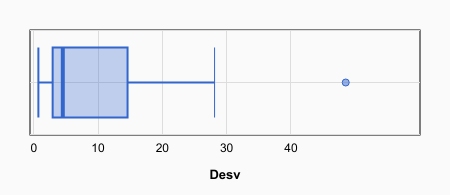
\includegraphics[scale=0.5]{boxplot-agepos-desv}
         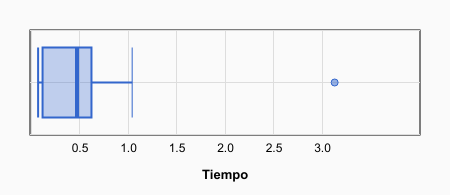
\includegraphics[scale=0.5]{boxplot-agepos-time}
      \end{center}
      
      
      \newpage
      \subsection{Resultados AGE con cruce OX}
      \begin{table}[H]
\centering
\label{my-label}
\begin{tabular}{|l|l|l|l|l|l|l|}
\hline
\multicolumn{7}{|c|}{\textbf{Algoritmo AGE-OX}}                                                                                                                                                                                                                   \\ \hline
\multicolumn{1}{|c|}{\textbf{Caso}} & \multicolumn{1}{c|}{\textbf{Desv}} & \multicolumn{1}{c|}{\textbf{Tiempo}} & \multicolumn{1}{c|}{\textbf{}} & \multicolumn{1}{c|}{\textbf{Caso}} & \multicolumn{1}{c|}{\textbf{Desv}} & \multicolumn{1}{c|}{\textbf{Tiempo}} \\ \cline{1-3} \cline{5-7} 
\textbf{Chr22a}                     & 25,41                              & 0,12                                 &                                & \textbf{Sko100a}                   & 12,82                              & 0,75                                 \\ \cline{1-3} \cline{5-7} 
\textbf{Chr22b}                     & 16,73                              & 0,12                                 &                                & \textbf{Sko100f}                   & 12,51                              & 0,73                                 \\ \cline{1-3} \cline{5-7} 
\textbf{Chr25a}                     & 121,29                             & 0,12                                 &                                & \textbf{Tai100a}                   & 11,77                              & 0,80                                 \\ \cline{1-3} \cline{5-7} 
\textbf{Esc128}                     & 93,75                              & 1,33                                 &                                & \textbf{Tai100b}                   & 28,43                              & 0,82                                 \\ \cline{1-3} \cline{5-7} 
\textbf{Had20}                      & 0,17                               & 0,12                                 &                                & \textbf{Tai150b}                   & 23,62                              & 1,56                                 \\ \cline{1-3} \cline{5-7} 
\textbf{Lipa60b}                    & 26,33                              & 0,41                                 &                                & \textbf{Tai256c}                   & 3,76                               & 3,54                                 \\ \cline{1-3} \cline{5-7} 
\textbf{Lipa80b}                    & 27,79                              & 0,59                                 &                                & \textbf{Tho40}                     & 22,94                              & 0,25                                 \\ \cline{1-3} \cline{5-7} 
\textbf{Nug28}                      & 7,70                               & 0,14                                 &                                & \textbf{Tho150}                    & 15,74                              & 1,38                                 \\ \cline{1-3} \cline{5-7} 
\textbf{Sko81}                      & 13,50                              & 0,58                                 &                                & \textbf{Wil50}                     & 7,70                               & 0,31                                 \\ \cline{1-3} \cline{5-7} 
\textbf{Sko90}                      & 13,54                              & 0,66                                 &                                & \textbf{Wil100}                    & 7,35                               & 0,77                                 \\ \cline{1-3} \cline{5-7} 
\end{tabular}
\end{table}

De nuevo, por las mismas razones que en apartado anterior, obtenemos mejores resultados en mejor tiempo que AGG OX. No obstante, debido a que el número de iteraciones es bajo, el cruce OX se comporta peor que el operador de cruce basado en posición.

\begin{center}
         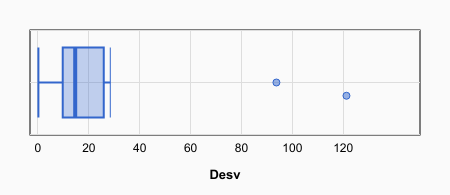
\includegraphics[scale=0.5]{boxplot-ageox-desv}
         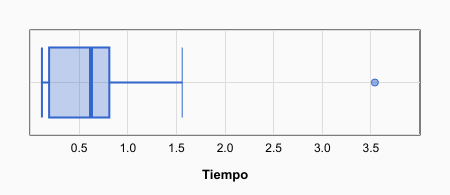
\includegraphics[scale=0.5]{boxplot-ageox-time}
      \end{center}
      
      
      
      \newpage
      \subsection{Resultados Memético (10, 1)}
      \begin{table}[H]
\centering
\label{my-label}
\begin{tabular}{|l|l|l|l|l|l|l|}
\hline
\multicolumn{7}{|c|}{\textbf{Algoritmo AM(10, 1)}}                                                                                                                                                                                                       \\ \hline
\multicolumn{1}{|c|}{\textbf{Caso}} & \multicolumn{1}{c|}{\textbf{Desv}} & \multicolumn{1}{c|}{\textbf{Tiempo}} & \multicolumn{1}{c|}{} & \multicolumn{1}{c|}{\textbf{Caso}} & \multicolumn{1}{c|}{\textbf{Desv}} & \multicolumn{1}{c|}{\textbf{Tiempo}} \\ \cline{1-3} \cline{5-7} 
\textbf{Chr22a}                     & 16,73                              & 0,07                                 &                       & \textbf{Sko100a}                   & 2,24                               & 0,60                                 \\ \cline{1-3} \cline{5-7} 
\textbf{Chr22b}                     & 19,66                              & 0,06                                 &                       & \textbf{Sko100f}                   & 1,60                               & 0,62                                 \\ \cline{1-3} \cline{5-7} 
\textbf{Chr25a}                     & 57,59                              & 0,07                                 &                       & \textbf{Tai100a}                   & 3,63                               & 0,58                                 \\ \cline{1-3} \cline{5-7} 
\textbf{Esc128}                     & 18,75                              & 0,78                                 &                       & \textbf{Tai100b}                   & 3,98                               & 0,73                                 \\ \cline{1-3} \cline{5-7} 
\textbf{Had20}                      & 0,40                               & 0,04                                 &                       & \textbf{Tai150b}                   & 3,19                               & 1,55                                 \\ \cline{1-3} \cline{5-7} 
\textbf{Lipa60b}                    & 20,49                              & 0,25                                 &                       & \textbf{Tai256c}                   & 0,64                               & 3,14                                 \\ \cline{1-3} \cline{5-7} 
\textbf{Lipa80b}                    & 21,68                              & 0,39                                 &                       & \textbf{Tho40}                     & 3,78                               & 0,13                                 \\ \cline{1-3} \cline{5-7} 
\textbf{Nug28}                      & 6,85                               & 0,07                                 &                       & \textbf{Tho150}                    & 2,96                               & 1,42                                 \\ \cline{1-3} \cline{5-7} 
\textbf{Sko81}                      & 2,20                               & 0,44                                 &                       & \textbf{Wil50}                     & 0,79                               & 0,18                                 \\ \cline{1-3} \cline{5-7} 
\textbf{Sko90}                      & 1,61                               & 0,52                                 &                       & \textbf{Wil100}                    & 0,72                               & 0,58                                 \\ \cline{1-3} \cline{5-7} 
\end{tabular}
\end{table}

	Al aplicar una búsqueda local sobre toda la población, en pocas iteraciones hemos mejorado mucho la calidad de nuestra población. Esto hace que los resultados sean mucho mejores que en AGG.\\

	Aplicar una búsqueda local sobre cada cromosoma es muy costoso, por lo tanto, para un mismo tamaño de población, un algoritmo memético tradará mas en completar una iteración que un Genético. Sin embargo, el tamaño de la población en nuestro experimento es 10, frente a los 50 del Genético por lo que no podemos apreciar este detalle. 



\begin{center}
         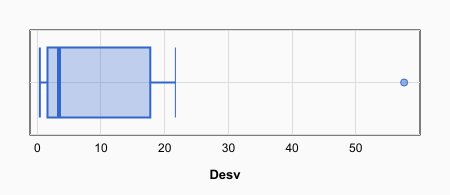
\includegraphics[scale=0.5]{boxplot-am(1-1)-desv}
         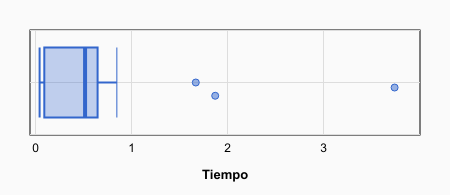
\includegraphics[scale=0.5]{boxplot-am(1-1)-time}
      \end{center}
      
      
      
      \newpage
      \subsection{Resultados Memético (10, 0.1)}
      \begin{table}[H]
\centering
\label{my-label}
\begin{tabular}{|l|l|l|l|l|l|l|}
\hline
\multicolumn{7}{|c|}{\textbf{Algoritmo AM(10, 0.1)}}                                                                                                                                                                                                     \\ \hline
\multicolumn{1}{|c|}{\textbf{Caso}} & \multicolumn{1}{c|}{\textbf{Desv}} & \multicolumn{1}{c|}{\textbf{Tiempo}} & \multicolumn{1}{c|}{} & \multicolumn{1}{c|}{\textbf{Caso}} & \multicolumn{1}{c|}{\textbf{Desv}} & \multicolumn{1}{c|}{\textbf{Tiempo}} \\ \cline{1-3} \cline{5-7} 
\textbf{Chr22a}                     & 11,57                              & 0,05                                 &                       & \textbf{Sko100a}                   & 2,00                               & 0,61                                 \\ \cline{1-3} \cline{5-7} 
\textbf{Chr22b}                     & 24,15                              & 0,05                                 &                       & \textbf{Sko100f}                   & 2,11                               & 0,55                                 \\ \cline{1-3} \cline{5-7} 
\textbf{Chr25a}                     & 42,15                              & 0,06                                 &                       & \textbf{Tai100a}                   & 4,44                               & 0,55                                 \\ \cline{1-3} \cline{5-7} 
\textbf{Esc128}                     & 15,63                              & 0,77                                 &                       & \textbf{Tai100b}                   & 4,99                               & 0,58                                 \\ \cline{1-3} \cline{5-7} 
\textbf{Had20}                      & 3,09                               & 0,04                                 &                       & \textbf{Tai150b}                   & 4,24                               & 1,21                                 \\ \cline{1-3} \cline{5-7} 
\textbf{Lipa60b}                    & 19,52                              & 0,24                                 &                       & \textbf{Tai256c}                   & 0,47                               & 3,07                                 \\ \cline{1-3} \cline{5-7} 
\textbf{Lipa80b}                    & 22,46                              & 0,39                                 &                       & \textbf{Tho40}                     & 5,42                               & 0,12                                 \\ \cline{1-3} \cline{5-7} 
\textbf{Nug28}                      & 7,47                               & 0,06                                 &                       & \textbf{Tho150}                    & 2,91                               & 1,16                                 \\ \cline{1-3} \cline{5-7} 
\textbf{Sko81}                      & 3,30                               & 0,42                                 &                       & \textbf{Wil50}                     & 2,53                               & 0,19                                 \\ \cline{1-3} \cline{5-7} 
\textbf{Sko90}                      & 3,32                               & 0,52                                 &                       & \textbf{Wil100}                    & 0,77                               & 0,56                                 \\ \cline{1-3} \cline{5-7} 
\end{tabular}
\end{table}

	Al aplicar la busqueda local sobre un porcentaje (en este caso 10\%) de la población mejoramos sustancialmente los resultados respecto a aplicar la búsqueda sobre todos los cromosomas. Esto se debe a que mantenemos mayor diversidad cuando ejecutamos la búsqueda local sobre solo un porcentaje.

\begin{center}
         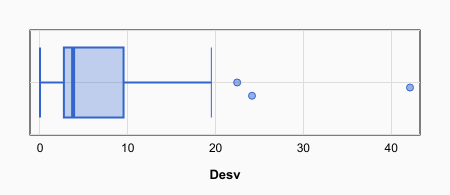
\includegraphics[scale=0.5]{boxplot-am(1-01)-desv}
         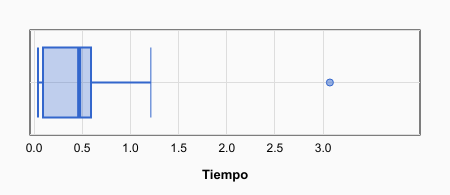
\includegraphics[scale=0.5]{boxplot-am(1-01)-time}
      \end{center}
      
      
      
      \newpage
      \subsection{Resultados Memético (10, 0.1 mejores)}
      \begin{table}[H]
\centering
\label{my-label}
\begin{tabular}{|l|l|l|l|l|l|l|}
\hline
\multicolumn{7}{|c|}{\textbf{Algoritmo AM(10, 0.1mej)}}                                                                                                                                                                                                     \\ \hline
\multicolumn{1}{|c|}{\textbf{Caso}} & \multicolumn{1}{c|}{\textbf{Desv}} & \multicolumn{1}{c|}{\textbf{Tiempo}} & \multicolumn{1}{c|}{} & \multicolumn{1}{c|}{\textbf{Caso}} & \multicolumn{1}{c|}{\textbf{Desv}} & \multicolumn{1}{c|}{\textbf{Tiempo}} \\ \cline{1-3} \cline{5-7} 
\textbf{Chr22a}                     & 18,84                              & 0,05                                 &                       & \textbf{Sko100a}                   & 1,52                               & 0,58                                 \\ \cline{1-3} \cline{5-7} 
\textbf{Chr22b}                     & 13,98                              & 0,05                                 &                       & \textbf{Sko100f}                   & 2,11                               & 0,57                                 \\ \cline{1-3} \cline{5-7} 
\textbf{Chr25a}                     & 48,05                              & 0,05                                 &                       & \textbf{Tai100a}                   & 4,16                               & 0,55                                 \\ \cline{1-3} \cline{5-7} 
\textbf{Esc128}                     & 12,50                              & 0,92                                 &                       & \textbf{Tai100b}                   & 1,80                               & 0,56                                 \\ \cline{1-3} \cline{5-7} 
\textbf{Had20}                      & 0,46                               & 0,04                                 &                       & \textbf{Tai150b}                   & 3,32                               & 1,27                                 \\ \cline{1-3} \cline{5-7} 
\textbf{Lipa60b}                    & 20,45                              & 0,27                                 &                       & \textbf{Tai256c}                   & 0,72                               & 2,89                                 \\ \cline{1-3} \cline{5-7} 
\textbf{Lipa80b}                    & 21,67                              & 0,50                                 &                       & \textbf{Tho40}                     & 4,18                               & 0,11                                 \\ \cline{1-3} \cline{5-7} 
\textbf{Nug28}                      & 5,46                               & 0,08                                 &                       & \textbf{Tho150}                    & 2,66                               & 1,16                                 \\ \cline{1-3} \cline{5-7} 
\textbf{Sko81}                      & 2,54                               & 0,46                                 &                       & \textbf{Wil50}                     & 2,19                               & 0,18                                 \\ \cline{1-3} \cline{5-7} 
\textbf{Sko90}                      & 1,79                               & 0,51                                 &                       & \textbf{Wil100}                    & 1,01                               & 0,52                                 \\ \cline{1-3} \cline{5-7} 
\end{tabular}
\end{table}

	De nuevo mejoramos aún mas los resultados obtenidos ya que mantenemos la diversidad pero mejoramos los mejores cromosomas aumentando rapidamente la calidad de nuestra población.

\begin{center}
         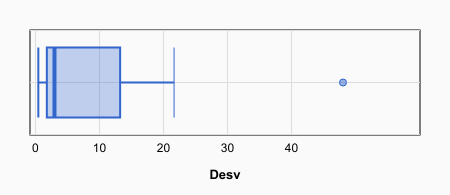
\includegraphics[scale=0.5]{boxplot-am(1-01mej)-desv}
         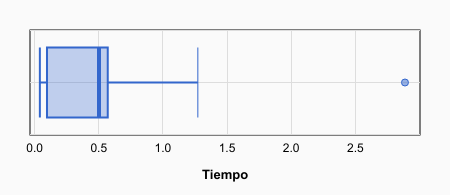
\includegraphics[scale=0.5]{boxplot-am(1-01mej)-time}
      \end{center}
      
      \newpage
      \subsection{Resultados Enfriamiento Simulado}
      \begin{table}[H]
\centering
\begin{tabular}{|l|l|l|l|l|l|l|}
\hline
\multicolumn{7}{|c|}{\textbf{ES - Cauchy}}                                                                          \\ \hline
\textbf{Caso}    & \textbf{Desv} & \textbf{Tiempo} & \textbf{} & \textbf{Caso}    & \textbf{Desv} & \textbf{Tiempo} \\ \cline{1-3} \cline{5-7} 
\textbf{Chr22a}  & 14,10         & 0,00            &           & \textbf{Sko100a} & 2,48          & 0,01            \\ \cline{1-3} \cline{5-7} 
\textbf{Chr22b}  & 13,56         & 0,00            &           & \textbf{Sko100f} & 1,73          & 0,04            \\ \cline{1-3} \cline{5-7} 
\textbf{Chr25a}  & 55,01         & 0,00            &           & \textbf{Tai100a} & 4,13          & 0,02            \\ \cline{1-3} \cline{5-7} 
\textbf{Esc128}  & 37,50         & 0,01            &           & \textbf{Tai100b} & 7,11          & 0,05            \\ \cline{1-3} \cline{5-7} 
\textbf{Had20}   & 1,39          & 0,00            &           & \textbf{Tai150b} & 2,61          & 0,06            \\ \cline{1-3} \cline{5-7} 
\textbf{Lipa60b} & 20,20         & 0,00            &           & \textbf{Tai256c} & 0,89          & 0,08            \\ \cline{1-3} \cline{5-7} 
\textbf{Lipa80b} & 21,85         & 0,01            &           & \textbf{Tho40}   & 4,26          & 0,00            \\ \cline{1-3} \cline{5-7} 
\textbf{Nug28}   & 4,22          & 0,00            &           & \textbf{Tho150}  & 2,77          & 0,07            \\ \cline{1-3} \cline{5-7} 
\textbf{Sko81}   & 2,07          & 0,01            &           & \textbf{Wil50}   & 1,20          & 0,00            \\ \cline{1-3} \cline{5-7} 
\textbf{Sko90}   & 2,29          & 0,02            &           & \textbf{Wil100}  & 1,47          & 0,01            \\ \cline{1-3} \cline{5-7} 
\end{tabular}
\end{table}

	Podemos ver que este algoritmo ofrece resultados bastante buenos rápidamente. Mejores incluso que la búsqueda local básica. Una vez más vemos que para problemas de QAP, las técnicas que se centran en explorar zonas concretas funcionan de media mejor que las que tienden a diversificar como los algoritmos genéticos o incluso meméticos.

	\begin{center}
         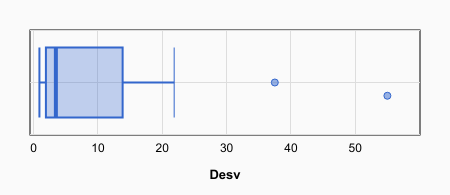
\includegraphics[scale=0.5]{desv-esCauchy}
         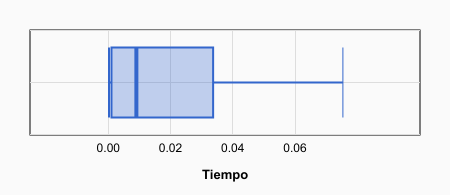
\includegraphics[scale=0.5]{time-esCauchy}
      \end{center}
      
      \begin{table}[H]
\centering
\begin{tabular}{|l|l|l|l|l|l|l|}
\hline
\multicolumn{7}{|c|}{\textbf{ES - Proporcional}}                                                                    \\ \hline
\textbf{Caso}    & \textbf{Desv} & \textbf{Tiempo} & \textbf{} & \textbf{Caso}    & \textbf{Desv} & \textbf{Tiempo} \\ \cline{1-3} \cline{5-7} 
\textbf{Chr22a}  & 44,87         & 0,01            &           & \textbf{Sko100a} & 13,93         & 0,05            \\ \cline{1-3} \cline{5-7} 
\textbf{Chr22b}  & 37,04         & 0,01            &           & \textbf{Sko100f} & 13,63         & 0,04            \\ \cline{1-3} \cline{5-7} 
\textbf{Chr25a}  & 163,33        & 0,01            &           & \textbf{Tai100a} & 12,32         & 0,04            \\ \cline{1-3} \cline{5-7} 
\textbf{Esc128}  & 265,63        & 0,06            &           & \textbf{Tai100b} & 36,65         & 0,04            \\ \cline{1-3} \cline{5-7} 
\textbf{Had20}   & 4,71          & 0,01            &           & \textbf{Tai150b} & 25,45         & 0,06            \\ \cline{1-3} \cline{5-7} 
\textbf{Lipa60b} & 27,20         & 0,03            &           & \textbf{Tai256c} & 11,20         & 0,15            \\ \cline{1-3} \cline{5-7} 
\textbf{Lipa80b} & 28,69         & 0,04            &           & \textbf{Tho40}   & 25,26         & 0,02            \\ \cline{1-3} \cline{5-7} 
\textbf{Nug28}   & 19,16         & 0,01            &           & \textbf{Tho150}  & 17,23         & 0,08            \\ \cline{1-3} \cline{5-7} 
\textbf{Sko81}   & 14,98         & 0,03            &           & \textbf{Wil50}   & 9,25          & 0,02            \\ \cline{1-3} \cline{5-7} 
\textbf{Sko90}   & 14,14         & 0,03            &           & \textbf{Wil100}  & 7,94          & 0,04            \\ \cline{1-3} \cline{5-7} 
\end{tabular}
\end{table}

	Podemos ver que los resultados obtenidos con este esquema de enfriamiento dejan mucho que desear.

	\begin{center}
         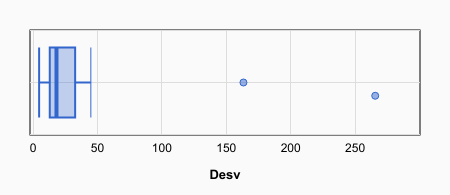
\includegraphics[scale=0.5]{desv-esProp}
         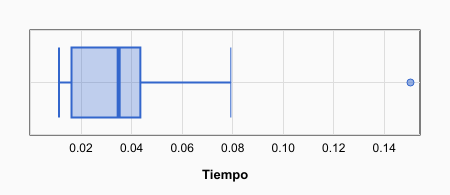
\includegraphics[scale=0.5]{time-esProp}
      \end{center}
      
      
      
      \newpage
      \subsection{Resultados Búsqueda Multiarranque Básica}
      \begin{table}[H]
      \centering
\begin{tabular}{|l|l|l|l|l|l|l|}
\hline
\multicolumn{7}{|c|}{\textbf{Búsqueda Multiarranque Básica}}                                                        \\ \hline
\textbf{Caso}    & \textbf{Desv} & \textbf{Tiempo} & \textbf{} & \textbf{Caso}    & \textbf{Desv} & \textbf{Tiempo} \\ \cline{1-3} \cline{5-7} 
\textbf{Chr22a}  & 17,45         & 0,00            &           & \textbf{Sko100a} & 2,87          & 0,02            \\ \cline{1-3} \cline{5-7} 
\textbf{Chr22b}  & 12,72         & 0,00            &           & \textbf{Sko100f} & 2,62          & 0,03            \\ \cline{1-3} \cline{5-7} 
\textbf{Chr25a}  & 77,56         & 0,00            &           & \textbf{Tai100a} & 3,89          & 0,02            \\ \cline{1-3} \cline{5-7} 
\textbf{Esc128}  & 6,25          & 0,03            &           & \textbf{Tai100b} & 5,45          & 0,04            \\ \cline{1-3} \cline{5-7} 
\textbf{Had20}   & 1,01          & 0,00            &           & \textbf{Tai150b} & 3,56          & 0,12            \\ \cline{1-3} \cline{5-7} 
\textbf{Lipa60b} & 20,38         & 0,00            &           & \textbf{Tai256c} & 0,67          & 0,20            \\ \cline{1-3} \cline{5-7} 
\textbf{Lipa80b} & 22,68         & 0,01            &           & \textbf{Tho40}   & 5,72          & 0,00            \\ \cline{1-3} \cline{5-7} 
\textbf{Nug28}   & 5,92          & 0,00            &           & \textbf{Tho150}  & 2,41          & 0,12            \\ \cline{1-3} \cline{5-7} 
\textbf{Sko81}   & 3,34          & 0,02            &           & \textbf{Wil50}   & 2,47          & 0,00            \\ \cline{1-3} \cline{5-7} 
\textbf{Sko90}   & 2,55          & 0,02            &           & \textbf{Wil100}  & 1,16          & 0,03            \\ \cline{1-3} \cline{5-7} 
\end{tabular}
\end{table}

	Aun tratándose de un algoritmo muy básico, consigue soluciones muy buenas. Sin embargo, es todo cuestión de suerte para generar soluciones iniciales aleatorias que se encuentren en zonas cercanas a óptimos locales buenos.

	\begin{center}
         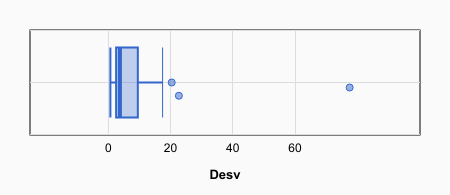
\includegraphics[scale=0.5]{desv-bmb}
         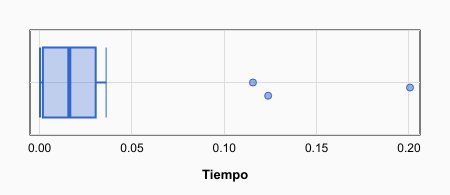
\includegraphics[scale=0.5]{time-bmb}
      \end{center}
      
      \newpage
      \subsection{Resultados GRASP}
      \begin{table}[H]
\centering
\begin{tabular}{|l|l|l|l|l|l|l|}
\hline
\multicolumn{7}{|c|}{\textbf{GRASP}}                                                                                \\ \hline
\textbf{Caso}    & \textbf{Desv} & \textbf{Tiempo} & \textbf{} & \textbf{Caso}    & \textbf{Desv} & \textbf{Tiempo} \\ \cline{1-3} \cline{5-7} 
\textbf{Chr22a}  & 9,52          & 0,00            &           & \textbf{Sko100a} & 2,26          & 0,22            \\ \cline{1-3} \cline{5-7} 
\textbf{Chr22b}  & 16,92         & 0,00            &           & \textbf{Sko100f} & 2,51          & 0,22            \\ \cline{1-3} \cline{5-7} 
\textbf{Chr25a}  & 42,10         & 0,00            &           & \textbf{Tai100a} & 3,47          & 0,21            \\ \cline{1-3} \cline{5-7} 
\textbf{Esc128}  & 3,13          & 0,53            &           & \textbf{Tai100b} & 7,19          & 0,23            \\ \cline{1-3} \cline{5-7} 
\textbf{Had20}   & 1,82          & 0,00            &           & \textbf{Tai150b} & 3,72          & 1,10            \\ \cline{1-3} \cline{5-7} 
\textbf{Lipa60b} & 20,15         & 0,04            &           & \textbf{Tai256c} & 0,49          & 7,92            \\ \cline{1-3} \cline{5-7} 
\textbf{Lipa80b} & 21,94         & 0,09            &           & \textbf{Tho40}   & 5,56          & 0,01            \\ \cline{1-3} \cline{5-7} 
\textbf{Nug28}   & 3,56          & 0,00            &           & \textbf{Tho150}  & 3,23          & 1,08            \\ \cline{1-3} \cline{5-7} 
\textbf{Sko81}   & 2,22          & 0,10            &           & \textbf{Wil50}   & 2,36          & 0,02            \\ \cline{1-3} \cline{5-7} 
\textbf{Sko90}   & 2,92          & 0,15            &           & \textbf{Wil100}  & 1,43          & 0,22            \\ \cline{1-3} \cline{5-7} 
\end{tabular}
\end{table}

	Soluciones muy buenas, que mejoran las del Enfriamiento simulado. La posibilidad de crear soluciones greedy no deterministas posibilita una explotación de diferentes zonas prometedoras que devuelven resultados muy cercanos al óptimo. 

	\begin{center}
         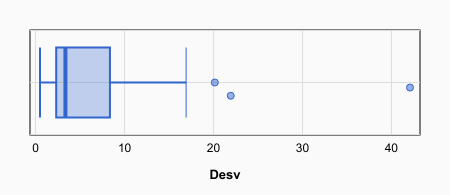
\includegraphics[scale=0.5]{desv-grasp}
         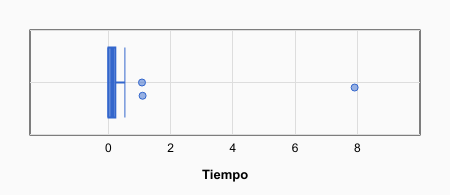
\includegraphics[scale=0.5]{time-grasp}
      \end{center}
      
      \newpage
      \subsection{Resultados ILS}
      \begin{table}[H]
\centering
\begin{tabular}{|l|l|l|l|l|l|l|}
\hline
\multicolumn{7}{|c|}{\textbf{ILS}}                                                                                  \\ \hline
\textbf{Caso}    & \textbf{Desv} & \textbf{Tiempo} & \textbf{} & \textbf{Caso}    & \textbf{Desv} & \textbf{Tiempo} \\ \cline{1-3} \cline{5-7} 
\textbf{Chr22a}  & 17,45         & 0,00            &           & \textbf{Sko100a} & 2,87          & 0,02            \\ \cline{1-3} \cline{5-7} 
\textbf{Chr22b}  & 12,72         & 0,00            &           & \textbf{Sko100f} & 2,62          & 0,02            \\ \cline{1-3} \cline{5-7} 
\textbf{Chr25a}  & 77,56         & 0,00            &           & \textbf{Tai100a} & 3,89          & 0,02            \\ \cline{1-3} \cline{5-7} 
\textbf{Esc128}  & 6,25          & 0,03            &           & \textbf{Tai100b} & 5,45          & 0,04            \\ \cline{1-3} \cline{5-7} 
\textbf{Had20}   & 1,01          & 0,00            &           & \textbf{Tai150b} & 3,56          & 0,12            \\ \cline{1-3} \cline{5-7} 
\textbf{Lipa60b} & 20,38         & 0,00            &           & \textbf{Tai256c} & 0,67          & 0,20            \\ \cline{1-3} \cline{5-7} 
\textbf{Lipa80b} & 22,68         & 0,01            &           & \textbf{Tho40}   & 5,72          & 0,00            \\ \cline{1-3} \cline{5-7} 
\textbf{Nug28}   & 5,92          & 0,00            &           & \textbf{Tho150}  & 2,41          & 0,12            \\ \cline{1-3} \cline{5-7} 
\textbf{Sko81}   & 3,34          & 0,01            &           & \textbf{Wil50}   & 2,47          & 0,00            \\ \cline{1-3} \cline{5-7} 
\textbf{Sko90}   & 2,55          & 0,02            &           & \textbf{Wil100}  & 1,16          & 0,03            \\ \cline{1-3} \cline{5-7} 
\end{tabular}
\end{table}

	Se trata de un algoritmo que mejora ligeramente a la búsqueda local. Obtenemos buenos resultados en poco tiempo. Si permitiésemos un mayor número de evaluaciones a costa de tiempo podriamos aproximarnos aún más a los resultados óptimos.

	\begin{center}
         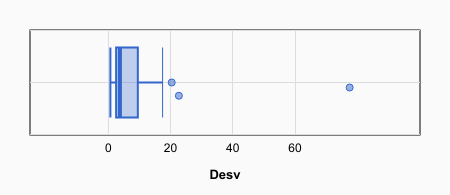
\includegraphics[scale=0.5]{desv-ils}
         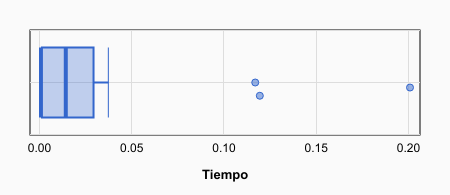
\includegraphics[scale=0.5]{time-ils}
      \end{center}

      
      \newpage
      \subsection{Resultados ILS-ES}
      \begin{table}[H]
\centering
\begin{tabular}{|l|l|l|l|l|l|l|}
\hline
\multicolumn{7}{|c|}{\textbf{ILS - ES Cauchy}}                                                                      \\ \hline
\textbf{Caso}    & \textbf{Desv} & \textbf{Tiempo} & \textbf{} & \textbf{Caso}    & \textbf{Desv} & \textbf{Tiempo} \\ \cline{1-3} \cline{5-7} 
\textbf{Chr22a}  & 6,40          & 0,03            &           & \textbf{Sko100a} & 1,47          & 0,67            \\ \cline{1-3} \cline{5-7} 
\textbf{Chr22b}  & 4,46          & 0,01            &           & \textbf{Sko100f} & 1,60          & 0,72            \\ \cline{1-3} \cline{5-7} 
\textbf{Chr25a}  & 27,56         & 0,02            &           & \textbf{Tai100a} & 3,73          & 0,47            \\ \cline{1-3} \cline{5-7} 
\textbf{Esc128}  & 0,00          & 0,34            &           & \textbf{Tai100b} & 0,90          & 0,95            \\ \cline{1-3} \cline{5-7} 
\textbf{Had20}   & 0,03          & 0,01            &           & \textbf{Tai150b} & 1,79          & 2,82            \\ \cline{1-3} \cline{5-7} 
\textbf{Lipa60b} & 19,80         & 0,12            &           & \textbf{Tai256c} & 0,60          & 3,35            \\ \cline{1-3} \cline{5-7} 
\textbf{Lipa80b} & 21,34         & 0,24            &           & \textbf{Tho40}   & 2,86          & 0,05            \\ \cline{1-3} \cline{5-7} 
\textbf{Nug28}   & 1,47          & 0,02            &           & \textbf{Tho150}  & 1,44          & 2,47            \\ \cline{1-3} \cline{5-7} 
\textbf{Sko81}   & 1,22          & 0,38            &           & \textbf{Wil50}   & 0,77          & 0,10            \\ \cline{1-3} \cline{5-7} 
\textbf{Sko90}   & 1,29          & 0,51            &           & \textbf{Wil100}  & 0,64          & 0,70            \\ \cline{1-3} \cline{5-7} 
\end{tabular}
\end{table}

	Estamos ante el algoritmo que mejores resultados ha obtenido, duplicando incluso la optimalidad de la búsqueda local. La capacidad de ILS para mutar y explorar nuevas zonas combinada con la capacidad de explotar dichas zonas moviéndose aleatoriamente por ella y dirigiéndose hacia el óptimo local del ES, hace que esta combinación usando el esquema de enfriamiento de Cauchy consiga resultados espectaculares en poco tiempo.

	\begin{center}
         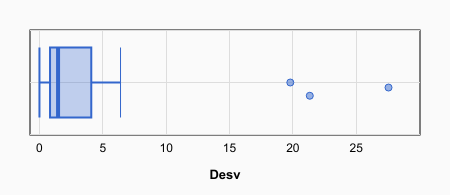
\includegraphics[scale=0.5]{desv-ilsEsCauchy}
         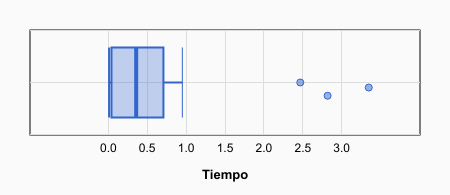
\includegraphics[scale=0.5]{time-ilsEsCauchy}
      \end{center}

\begin{table}[H]
\centering
\begin{tabular}{|l|l|l|l|l|l|l|}
\hline
\multicolumn{7}{|c|}{\textbf{ILS - ES Proporcional}}                                                                \\ \hline
\textbf{Caso}    & \textbf{Desv} & \textbf{Tiempo} & \textbf{} & \textbf{Caso}    & \textbf{Desv} & \textbf{Tiempo} \\ \cline{1-3} \cline{5-7} 
\textbf{Chr22a}  & 33,63         & 0,53            &           & \textbf{Sko100a} & 12,34         & 1,76            \\ \cline{1-3} \cline{5-7} 
\textbf{Chr22b}  & 25,22         & 0,51            &           & \textbf{Sko100f} & 12,99         & 1,90            \\ \cline{1-3} \cline{5-7} 
\textbf{Chr25a}  & 163,33        & 0,57            &           & \textbf{Tai100a} & 11,58         & 1,80            \\ \cline{1-3} \cline{5-7} 
\textbf{Esc128}  & 221,88        & 2,47            &           & \textbf{Tai100b} & 33,40         & 1,77            \\ \cline{1-3} \cline{5-7} 
\textbf{Had20}   & 2,92          & 0,49            &           & \textbf{Tai150b} & 23,84         & 3,21            \\ \cline{1-3} \cline{5-7} 
\textbf{Lipa60b} & 26,33         & 1,05            &           & \textbf{Tai256c} & 9,66          & 6,90            \\ \cline{1-3} \cline{5-7} 
\textbf{Lipa80b} & 28,14         & 1,36            &           & \textbf{Tho40}   & 21,01         & 0,73            \\ \cline{1-3} \cline{5-7} 
\textbf{Nug28}   & 14,75         & 0,59            &           & \textbf{Tho150}  & 16,68         & 2,92            \\ \cline{1-3} \cline{5-7} 
\textbf{Sko81}   & 14,01         & 1,40            &           & \textbf{Wil50}   & 8,41          & 0,87            \\ \cline{1-3} \cline{5-7} 
\textbf{Sko90}   & 13,50         & 1,57            &           & \textbf{Wil100}  & 7,35          & 1,93            \\ \cline{1-3} \cline{5-7} 
\end{tabular}
\end{table}

	De nuevo, por las mismas razones que en el enfriamiento simulado, es esquema de enfriamiento proporcional no ofrece buenos resultados.

	\begin{center}
         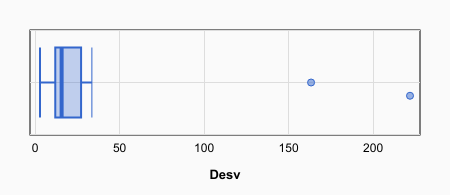
\includegraphics[scale=0.5]{desv-ilsEsProp}
         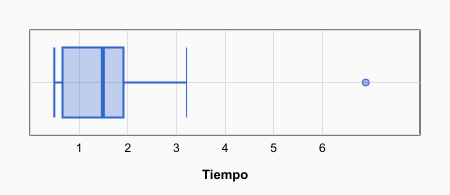
\includegraphics[scale=0.5]{time-ilsEsProp}
      \end{center}
      
      
      
      
      \newpage
      \subsection{Comparación de los resultados. Conclusiones.}
\begin{table}[H]
\centering
\label{my-label}
\begin{tabular}{|l|l|l|}
\hline
\multicolumn{1}{|c|}{\textbf{Algoritmo}} & \textbf{Desv} & \multicolumn{1}{c|}{\textbf{Tiempo}} \\ \hline
\textbf{Greedy}                          & 61,08         & 0,00088787315                        \\ \hline
\textbf{BL}                              & 10,66         & 2,80                                 \\ \hline
\textbf{BL. Don't Look Bits}             & 8.26          & 0,33                                 \\ \hline
\end{tabular}
\end{table}
      
      Como podemos ver, el tiempo de ejecución del algoritmo greedy es varias magnitudes menor que los tiempos de los otros dos algoritmos. Sin embargo, la poca calidad de sus soluciones hace que, por si sola, no sea una herramienta idónea de cara a resolver problemas.\\
      
      Tanto la Búsqueda Local básica como su variante con \textit{Dont't look bits} nos ofrecen resultados mucho mas óptimos que el greedy. \\
      
      Como la desviación de BL y BL con DLB es similar, debemos fijarnos en el tiempo medio de ejecución. La variante \textit{DLB} es 8.5 veces más rápida\footnote{$2.80/0.33 = 8.\overline{48}$} que la original. Aunque la variante \textit{Don't Look Bits} ofrece resultados ligeramente mejores, esto no debe ser tomado como referencia, pues la naturaleza aleatoria de cara a generar la solución de partida hace que no podamos asegurar que uno encuentra siempre una solución mejor que la otra.\\
      
      Cabe destacar que el experimento ha sido compilado sin optimización (\textbf{\textit{Debug}}). La realidad es que con un nivel máximo de optimización (\textbf{\textit{Release}}), aún en problemas de mayor tamaño y complejidad como \textbf{\textit{Tai150b}} obtenemos unos tiempos mucho menores que hace que utilizar un greedy en producción sea aun menos viable.\\
      
      Un ejemplo ilustrativo de la diferencia de tiempos en función del nivel de optimización:
      
\begin{table}[H]
\centering
\label{my-label}
\begin{tabular}{l|c|c|}
\cline{2-3}
\multicolumn{1}{c|}{{\textit{Tai150b}}} & \multicolumn{2}{c|}{\textbf{Nivel de Optimización}} \\ \hline
\multicolumn{1}{|c|}{\textbf{Algoritmo}}    & \textbf{Debug}          & \textbf{Release}          \\ \hline
\multicolumn{1}{|l|}{\textbf{BL}}           & 24.174                  & 1.55584                   \\ \hline
\multicolumn{1}{|l|}{\textbf{BL DLB}}       & 1.54554                 & 0.105939                  \\ \hline
\end{tabular}
\end{table}

	\newpage
	\begin{table}[H]
\centering
\label{my-label}
\begin{tabular}{|l|l|l|}
\hline
\textbf{Algoritmo}            & \textbf{Desv} & \textbf{Tiempo} \\ \hline
\textbf{Greedy}               & 61.08         & 0,0000609593    \\ \hline
\textbf{BL}                   & 10.66         & 0.24            \\ \hline
\textbf{BL. DLB}              & 8.26          & 0,03            \\ \hline
\textbf{AGG. Posición}        & 11.55         & 0,66            \\ \hline
\textbf{AGG. OX}              & 26,76         & 0,84            \\ \hline
\textbf{AGE. Posición}        & 10,11         & 0,56            \\ \hline
\textbf{AGE. OX}              & 24,64         & 0,76            \\ \hline
\textbf{AM (10, 1)}           & 9,48          & 0,61            \\ \hline
\textbf{AM (10, 0.1)}         & 9.13          & 0,56            \\ \hline
\textbf{AM (10, 0.1 mejores)} & 8,47          & 0,57            \\ \hline
\end{tabular}
\end{table}

	Como podemos ver, aunque obtenemos resultados bastante buenos, ninguno mejora la búsqueda local. 
	Si bien los algoritmos genéticos y los meméticos son planteamientos mucho más sofisticados que la búsqueda local, necesitan ser ajustandos correctamente para su correcto funcionamiento:\\
	
	\begin{itemize}
		\item En el caso de los genéticos, podemos jugar con el tamaño de la población y el número máximo de evaluaciones.\\
	
		\item En el caso de los meméticos, podemos ajustar los mismo parámetros que en los genéticos y, además, cada cuanto ejecutar la búsqueda local y sobre que cromosomas.\\
	\end{itemize}
	
	Hay que tener muy en cuenta el tiempo a la hora de ajustar estos parámetros pues por ejemplo ejecutar una búsqueda local sobre todos los cromosomas de una población de tamaño 100 es muy costoso y podemos conseguir el mismo resultado calibrando el porcentaje sobre los que ejecutar la búsqueda y el número máximo de evaluaciones.\\
	
	\newpage
	En el siguiente gráfico, podemos ver como evolucionan los algoritmos en función del número máximo de evaluaciones. Sobra decir que a mayor límite de evaluaciones mayor tiempo se necesita.\\
	
	\begin{center}
         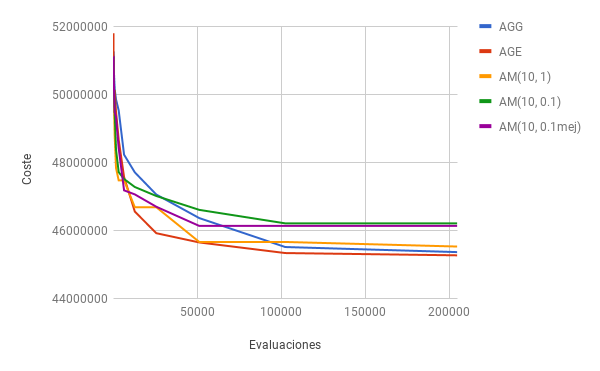
\includegraphics[scale=0.7]{evals-vs-coste}
      \end{center}
      
      Como vemos a mayor número de evaluaciones máximas, mejores resultados. Con un número de evaluaciones máximas los suficientemente grandes, los meméticos funcionan mejor que los genéticos pero se quedan estancados. Esto hace que para un número de evaluaciones aún mayor, los AGE obtengan (en un tiempo menor) mejores resultados que los AGG y parecidos al memetico que aplica BL sobre toda la población.\\
      
      Como conclusión final sobre los algorítmos genéticos y meméticos, cabe destacar que para el problema de QAP, los resultados que obtenemos con los genéticos al incrementar el número de evaluaciones máximas respecto del tiempo no son buenas. Esto se debe a que estos algoritmos no se comportan bien con codificaciones de orden. Aunque localizan zonas prometedoras, no son capaces de explorarlas bien; es por esto que los meméticos permiten obtener los mejores resultados en estos problemas. Un memético bien afinado, con un número suficiente de evaluaciones máximas y un buen equilibrio con la búsqueda local es una solucion muy buena para este tipo de problemas. 
      
      \newpage
      \begin{table}[H]
\centering
\begin{tabular}{|l|l|l|}
\hline
\multicolumn{1}{|c|}{\textbf{Algortimo}} & \multicolumn{1}{c|}{\textbf{Desv}} & \multicolumn{1}{c|}{\textbf{Tiempo}} \\ \hline
\textbf{Greedy}                          & 61.08                              & 0.00                                 \\ \hline
\textbf{BL}                              & 10.66                              & 0.24                                 \\ \hline
\textbf{ES}                              & 10,04                              & 0,02                                 \\ \hline
\textbf{BMB}                             & 10,03                              & 0,03                                 \\ \hline
\textbf{GRASP}                           & 7,82                               & 0,61                                 \\ \hline
\textbf{ILS}                             & 10,03                              & 0.03                                 \\ \hline
\textbf{ILS - ES}                        & 4,97                               & 0,70                                 \\ \hline
\end{tabular}
\end{table}
      
      En la anterior tabla comparamos los resultados de los algoritmos basados en trayectorias. Como podemos ver, hemos conseguido muy buenos resultados ya que como hemos comentado anteriormente, en los problemas basados en codificaciones de orden lo que mejor funciona es explotar más que diversificar. Esto no significa que no haya que diversificar, de hecho, la principal razón por la cual ILS-ES o GRASP funciona tan bien es por que tiene muy buen equilibrio entre diversificación y explotación.\\
      
      Como conclusión, podemos extraer que no por tener un algoritmo más sofisticado (AG y AM) vamos a obtener mejores resultados. Antes de ponernos a programar, debemos entender la naturaleza de nuestro problema y valorar los pros y contras de utilizar una familia de metaheurísticas u otras. 	
   
\printindex
\end{document}
